\PassOptionsToPackage{unicode=true}{hyperref} % options for packages loaded elsewhere
\PassOptionsToPackage{hyphens}{url}
%
\documentclass[12pt,]{article}
\usepackage{lmodern}
\usepackage{amssymb,amsmath}
\usepackage{ifxetex,ifluatex}
\usepackage{fixltx2e} % provides \textsubscript
\ifnum 0\ifxetex 1\fi\ifluatex 1\fi=0 % if pdftex
  \usepackage[T1]{fontenc}
  \usepackage[utf8]{inputenc}
  \usepackage{textcomp} % provides euro and other symbols
\else % if luatex or xelatex
  \usepackage{unicode-math}
  \defaultfontfeatures{Ligatures=TeX,Scale=MatchLowercase}
\fi
% use upquote if available, for straight quotes in verbatim environments
\IfFileExists{upquote.sty}{\usepackage{upquote}}{}
% use microtype if available
\IfFileExists{microtype.sty}{%
\usepackage[]{microtype}
\UseMicrotypeSet[protrusion]{basicmath} % disable protrusion for tt fonts
}{}
\IfFileExists{parskip.sty}{%
\usepackage{parskip}
}{% else
\setlength{\parindent}{0pt}
\setlength{\parskip}{6pt plus 2pt minus 1pt}
}
\usepackage{hyperref}
\hypersetup{
            pdftitle={Compositional stability of sediment microbial communities during a seagrass meadow decline},
            pdfborder={0 0 0},
            breaklinks=true}
\urlstyle{same}  % don't use monospace font for urls
\usepackage[margin=1.0in]{geometry}
\usepackage{graphicx,grffile}
\makeatletter
\def\maxwidth{\ifdim\Gin@nat@width>\linewidth\linewidth\else\Gin@nat@width\fi}
\def\maxheight{\ifdim\Gin@nat@height>\textheight\textheight\else\Gin@nat@height\fi}
\makeatother
% Scale images if necessary, so that they will not overflow the page
% margins by default, and it is still possible to overwrite the defaults
% using explicit options in \includegraphics[width, height, ...]{}
\setkeys{Gin}{width=\maxwidth,height=\maxheight,keepaspectratio}
\setlength{\emergencystretch}{3em}  % prevent overfull lines
\providecommand{\tightlist}{%
  \setlength{\itemsep}{0pt}\setlength{\parskip}{0pt}}
\setcounter{secnumdepth}{0}
% Redefines (sub)paragraphs to behave more like sections
\ifx\paragraph\undefined\else
\let\oldparagraph\paragraph
\renewcommand{\paragraph}[1]{\oldparagraph{#1}\mbox{}}
\fi
\ifx\subparagraph\undefined\else
\let\oldsubparagraph\subparagraph
\renewcommand{\subparagraph}[1]{\oldsubparagraph{#1}\mbox{}}
\fi

% set default figure placement to htbp
\makeatletter
\def\fps@figure{htbp}
\makeatother

\usepackage{times} % Times New Roman font
\usepackage[T1]{fontenc}

\usepackage[none]{hyphenat}

\usepackage{setspace}
\doublespacing
\setlength{\parskip}{1em}

\usepackage{lineno}
\renewcommand{\linenumberfont}{\normalfont\tiny}

\usepackage{pdfpages}

\usepackage{indentfirst}

\usepackage[labelsep=period, labelfont=bf]{caption}
\renewcommand{\thefigure}{\arabic{figure}}
\renewcommand{\figurename}{Figure}
\captionsetup{justification=raggedright,singlelinecheck=false}

\usepackage{pdflscape}
\newcommand{\blandscape}{\begin{landscape}}
\newcommand{\elandscape}{\end{landscape}}

\usepackage{siunitx}
\DeclareSIUnit\molar{\mole\per\cubic\deci\metre}
\DeclareSIUnit\Molar{\textsc{m}}
\DeclareSIUnit\cells{\text{cells}}
\DeclareSIUnit\litre{l}

\usepackage{caption}
\captionsetup{justification=justified}

\usepackage{float}

\usepackage{xr}
\externaldocument[supp-]{supplementary}

\usepackage{txfonts}

\renewcommand{\figureautorefname}{Figure}

\usepackage{microtype}

\usepackage{chemformula}

\title{\textbf{Compositional stability of sediment microbial communities during
a seagrass meadow decline}}
\author{}
\date{\vspace{-2.5em}}

\begin{document}
\maketitle

\vspace{20mm}

Marsej Markovski\textsuperscript{1}, Mirjana Najdek\textsuperscript{1},
Gerhard J. Herndl\textsuperscript{2,3}, and Marino
Korlević\textsuperscript{1\(*\)}

1. Center for Marine Research, Ruđer Bošković Institute, Croatia

2. Department of Functional and Evolutionary Ecology, University of
Vienna, Austria

3. Department of Marine Microbiology and Biogeochemistry, Royal
Netherlands Institute for Sea Research (NIOZ), Utrecht University, The
Netherlands

\textsuperscript{\(*\)}To whom correspondence should be addressed:

Marino Korlević

G. Paliaga 5, 52210 Rovinj, Croatia

Tel.: +385 52 804 768

Fax: +385 52 804 780

e-mail:
\href{mailto:marino.korlevic@irb.hr}{\nolinkurl{marino.korlevic@irb.hr}}

Running title: Compositional stability of sediment communities

\newpage
\linenumbers
\sisetup{mode=text}
\setlength\parindent{24pt}

\hypertarget{abstract}{%
\subsection{Abstract}\label{abstract}}

The presence of seagrass shapes surface sediments and forms a specific
environment for diverse and abundant microbial communities. A severe
decline of \emph{Cymodocea nodosa}, a widespread seagrass species in the
Mediterranean Sea, has been documented. To characterise and assess the
changes in microbial community composition during the decline of a
\emph{Cymodocea nodosa} meadow, Illumina MiSeq sequencing of the V4
region of the 16S rRNA gene was performed. Samples of surface sediments
were collected at monthly intervals from July 2017 to October 2018.
Samples from an adjacent, nonvegetated site were also analysed for
comparison. Microbial communities were stratified by sediment depth and
differed between the vegetated and the nonvegetated site. Although the
\emph{C. nodosa} meadow declined to a point where almost no leaves were
present, no clear temporal succession in the community was observed.
Taxonomic analysis revealed a dominance of bacterial over archaeal
sequences, with most archaeal reads classified as \emph{Nanoarchaeota},
\emph{Thermoplasmatota}, \emph{Crenarchaeota}, and
\emph{Asgardarchaeota}. The bacterial community was mainly composed of
\emph{Desulfobacterota}, \emph{Gammaproteobacteria},
\emph{Bacteroidota}, \emph{Chloroflexi}, \emph{Planctomycetota}, and
\emph{Campylobacterota}. Our results show that sediment microbial
communities are remarkably stable and may resist major disturbances such
as seagrass meadow decline.

\newpage

\hypertarget{introduction}{%
\subsection{Introduction}\label{introduction}}

Shallow coastal sediments are often colonized by seagrasses, which cover
approximately 0.1 to 0.2 \% of the global ocean (Duarte, 2002).
Seagrasses penetrate the sediment with their roots and rhizomes forming
extensive meadows. The presence of seagrass meadows shapes surface
sediments and provides a specific environment for diverse and abundant
microbial communities (Duarte et al., 2005). Sediments colonized by
seagrasses are considered hotspots for microbial activity as seagrass
meadows enrich the underlying sediment with organic matter (Duarte et
al., 2005). High organic matter content is mainly achieved by releasing
dissolved organic carbon from seagrass roots and by trapping organic
particles from the water column (Duarte, 2002). Moreover, seagrasses
stabilize the underlying sediment, promoting the accumulation of organic
matter and sediment particles (Fonseca and Kenworthy, 1987; Terrados and
Duarte, 2000; van Katwijk et al., 2010). In addition, seagrass beds can
also increase the availability of organic matter indirectly through the
decomposition of detached leaves, roots and rhizomes (Jensen et al.,
2007; Liu et al., 2017).

Studies of marine sediment microbial communities primarily focus on
changes in microbial abundance and activity with sediment depth
(Jørgensen and Marshall, 2016; Petro et al., 2017; Starnawski et al.,
2017; Orsi, 2018). Depth-dependent changes in taxonomic composition have
been well described differentiating surface sediment communities
dominated by \emph{Bacteria}, especially \emph{Proteobacteria}, from
deeper communities characterized by \emph{Archaea} (Orcutt et al., 2011;
Chen et al., 2017; Petro et al., 2017). Coastal surface sediments
colonized by seagrass are not as well investigated due to studies
focusing primarily on rhizosphere communities and only occasionally
including sediment communities for comparison (Cúcio et al., 2016;
Rabbani et al., 2021). Communities in the rhizosphere are
species-specific and differ from those in the sediment. One of the main
differences is the higher relative abundance of \emph{Desulfobacterota},
one of the most abundant sulphate reducing bacteria in seagrass
sediments, in contrast to the rhizosphere, which is characterized by
\emph{Epsilonproteobacteria} (Ettinger et al., 2017). When sediment
microbial communities were described, the main focus was on the
differences between vegetated and nonvegetated sites (Zheng et al.,
2019; Sun et al., 2020). In addition, these studies showed that
communities differ even with respect to the meadow edge (Ettinger et
al., 2017). However, little is known about the response of these
communities to seagrass decline. Only limited information is available
on the succession of microbial communities in seagrass sediments
including the dynamics and activity of sulphate-reducing prokaryotes
(Smith et al., 2004), the response of microbial communities to nutrient
enrichment (Guevara et al., 2014), and community changes associated with
seagrass restoration (Bourque et al., 2015). These studies suggest that
seagrass decline may trigger changes in the sediment communities.

In the Mediterranean Sea, \emph{Cymodocea nodosa} is a widespread
seagrass species declining in coastal areas (Ruiz Fernandez et al.,
2009; Tuya et al., 2014; Orlando-Bonaca et al., 2015). The rhizosphere
and epiphytic communities of \emph{C. nodosa} have been described (Cúcio
et al., 2016; Korlević et al., 2021a), however, little is known about
sediment communities underlying \emph{C. nodosa} meadows. The aim of the
present study was to characterize the taxonomic composition of sediment
communities of a \emph{C. nodosa} meadow and to assess the temporal
dynamics of these communities. As the studied meadow experienced a major
decline (Najdek et al., 2020), we investigated whether this event
affected the sediment microbial community structure.

\newpage

\hypertarget{materials-and-methods}{%
\subsection{Materials and methods}\label{materials-and-methods}}

\hypertarget{sampling}{%
\subsubsection{Sampling}\label{sampling}}

Sediment cores were sampled in a declining \emph{C. nodosa} meadow
(vegetated site) located in the Bay of Saline, east coast of the
northern Adriatic Sea (\ang{45;7;5} N, \ang{13;37;20} E)
(\autoref{map}). Cores were collected monthly from July 2017 to October
2018 (Supplementary \autoref{supp-nseq_notus}) by diving using 15 cm
long plastic core samplers. Sediment samples were immediately
transported on ice to the laboratory and stored at \num{-80}
\si{\degreeCelsius} until further processing. The adjacent nonvegetated
area was also sampled for comparison (\autoref{map}). A detailed
description of the study site, the decline of the \emph{C. nodosa}
meadow and the dynamics of environmental conditions during the decline
are provided in Najdek et al. (2020).

\hypertarget{dna-isolation}{%
\subsubsection{DNA isolation}\label{dna-isolation}}

Total DNA from sediment samples was extracted following a modified
(Pjevac et al., 2018) isolation protocol of Zhou et al. (1996). Prior to
DNA isolation, cores were cut into four different 1 \si{\cm} sections:
top (0 -- 1 \si{\cm}), bottom (7 -- 8 \si{\cm}), and two middle
sections: upper middle (1 -- 3 \si{\cm}) and lower middle (3 -- 6
\si{\cm}) section. Sediment samples were weighted (2 \si{\g}) avoiding
roots and rhizomes from vegetated cores, mixed with 5.4 \si{\ml} of
extraction buffer (100 \si{\milli\Molar} Tris {[}pH 8.0{]}, 100
\si{\milli\Molar} sodium EDTA {[}pH 8.0{]}, 100 \si{\milli\Molar}
\ch{Na3PO4} {[}pH 8.0{]}, 1.5 \si{\Molar} NaCl, 1 \si{\percent} CTAB)
and 10 \si{\ul} of proteinase K (20 \si{\mg\per\ml}) and incubated by
horizontal shaking at 225 rpm at 37\si{\degreeCelsius} for 30
\si{\minute}. Thereafter 1.2 \si{\ml} of 10 \si{\percent} SDS was added
and the mixture incubated again by horizontal shaking at 225 rpm at
65\si{\degreeCelsius} for 60 \si{\minute}. The supernatant was collected
after centrifugation at 3220 × g at room temperature for 10 \si{\minute}
and mixed with an equal volume of chloroform:isoamyl alcohol (1:1). The
aqueous phase was retrieved after centrifugation at 3220 × g at room
temperature for 10 \si{\minute}. The extraction procedure with the
organic solvent mixture was repeated twice. After the final extraction
0.6 volumes of isopropanol were added to precipitate the DNA. The
mixture was incubated at 22\si{\degreeCelsius} for 60 \si{\minute} and
centrifuged at 3220 × g at room temperature for 45 \si{\minute}. The
obtained pellet was washed twice with 10 \si{\ml} of chilled 70
\si{\percent} ethanol, centrifuged at 3220 × g at room temperature for
10 \si{\minute} after each washing, and finally resuspended in 100
\si{\ul} of deionized water.

\hypertarget{illumina-16s-rrna-sequencing}{%
\subsubsection{Illumina 16S rRNA
sequencing}\label{illumina-16s-rrna-sequencing}}

The V4 region of the 16S rRNA gene was sequenced using a two-step PCR
approach described previously (Korlević et al., 2021b). Briefly, the V4
region was amplified using the 515F (\(5'\)-GTGYCAGCMGCCGCGGTAA-\(3'\))
and 806R (\(5'\)-GGACTACNVGGGTWTCTAAT-\(3'\)) primers from the Earth
microbiome project
(\url{https://earthmicrobiome.org/protocols-and-standards/16s/}), which
contained a sequence tag on the 5' end (Caporaso et al., 2011, 2012;
Apprill et al., 2015; Parada et al., 2016). Purified samples were sent
for Illumina MiSeq sequencing (2 × 250 bp) at IMGM Laboratories
(Martinsried, Germany) where the second PCR of the two-step PCR approach
was performed using primers targeting the tag region incorporated in the
first PCR. These primers also contained adapter and sample-specific
index sequences. For each sequencing batch, a positive and a negative
control were also sequenced. The positive control consisted of a mock
community composed of uniformly mixed DNA from 20 different bacterial
strains (ATCC MSA-1002, ATCC, USA), while PCR reactions without DNA
template served as the negative control. Sequences obtained in this
study have been deposited in the European Nucleotide Archive at EMBL-EBI
under the accession numbers SAMEA11293274 -- SAMEA11293412 and
SAMEA6648825.

\hypertarget{sequence-and-data-analysis}{%
\subsubsection{Sequence and data
analysis}\label{sequence-and-data-analysis}}

Sequences were analysed on the computer cluster Isabella (University
Computing Center, University of Zagreb) using version 1.45.2 of mothur
(Schloss et al., 2009) according to the MiSeq Standard Operating
Procedure (MiSeq SOP; \url{https://mothur.org/wiki/miseq_sop/}) (Kozich
et al., 2013) and recommendations given by the Riffomonas project
(\url{https://riffomonas.org}) to foster data reproducibility. Alignment
and classification were performed using the 138.1 release of the SILVA
SSU Ref NR 99 database (\url{https://www.arb-silva.de}) (Quast et al.,
2013; Yilmaz et al., 2014). A cut-off of 97 \% was used to cluster
sequences into operational taxonomic units (OTUs).

Pipeline data processing and visualization were done using R (version
3.6.3) (R Core Team, 2020) combined with packages vegan (version 2.5.7)
(Oksanen et al., 2020) tidyverse (version 1.3.1) (Wickham et al., 2019)
and multiple other packages (Neuwirth, 2014; Xie, 2014, 2015, 2019,
2021a, 2021b; Xie et al., 2018, 2020; Edwards, 2020; Wilke, 2020;
Allaire et al., 2021; Zhu, 2021). Observed number of OTUs, Chao1, ACE,
exponential of the Shannon diversity index and Inverse Simpson diversity
index were calculated after normalization to the minimum number of reads
per sample to account for different sequencing depths using vegan's
function \texttt{rrarefy} (Oksanen et al., 2020). Chao1 and ACE
estimators were calculated using vegan's function \texttt{estimateR},
while Shannon and Inverse Simpson diversity indices were obtained using
vegan's function \texttt{diversity} (Oksanen et al., 2020). To express
both diversity indices in terms of effective number of OTUs the
exponential of the Shannon diversity index was retrieved (Jost, 2006).
The proportions of shared community members between different sediment
layers and the two sites were expressed as the Bray-Curtis similarity
coefficient calculated on the OTU data table using vegan's function
\texttt{vegdist} and transformed from dissimilarities to similarities
(Legendre and Legendre, 2012; Borcard et al., 2018; Oksanen et al.,
2020). The Principal Coordinate Analysis (PCoA) was performed on
Bray-Curtis dissimilarities based on OTU abundances using the function
\texttt{wcmdscale} (Legendre and Legendre, 2012; Oksanen et al., 2020).
Differences between communities of different layers, sites, years, and
decay periods were tested by performing the Analysis of Similarities
(ANOSIM) using vegan's function \texttt{anosim} and 1000 permutations
(Oksanen et al., 2020). In addition, differences between richness
estimators, diversity indices, and relative sequence abundances were
tested by performing the Mann-Whitney \emph{U} test (function
\texttt{wilcox.test}), when two groups were compared, or the
Kruskal-Wallis \emph{H} test (function \texttt{kruskal.test}) followed
by a pairwise comparison using the Mann-Whitney \emph{U} test (function
\texttt{pairwise.wilcox.test}), when more than two groups were compared.
Bonferroni correction was applied to address the problem of multiple
comparisons.

In total 3.3 million sequences were obtained after quality curation and
exclusion of sequences without known relatives (no relative sequences),
and eukaryotic, chloroplast, and mitochondrial sequences. Altogether, 68
samples from the vegetated sediment and 68 from the nonvegetated
sediment were analysed. The number of reads per sample ranged from 9,722
to 55,381 (Supplementary \autoref{supp-nseq_notus}). Even with the
highest sequencing effort the rarefaction curves did not level off as
commonly observed in high-throughput 16S rRNA amplicon sequencing
approaches (Supplementary \autoref{supp-rarefaction_a}, and
\ref{supp-rarefaction_b}). After quality curation and exclusion of
sequences as mentioned above, reads were clustered into 89,488 different
OTUs. Normalization to the minimum number of sequences (9,722) described
earlier resulted in 64,335 distinct OTUs ranging from 1,774 to 3,576
OTUs per sample (Supplementary \autoref{supp-estimators_moths}). Based
on the positive control, a sequencing error rate of 0.01 \si{\percent}
was calculated which is in line with previously reported values for
high-throughput sequencing data (Kozich et al., 2013; Schloss et al.,
2016). Following quality curation, the negative controls yielded on
average 34.2 ± 62.6 sequences. The detailed analysis procedure is
available in a Github repository
(\url{https://github.com/MicrobesRovinj/Markovski_SalineSediment16S_x_2022}).

\newpage

\hypertarget{results}{%
\subsection{Results}\label{results}}

To assess the richness and diversity of microbial communities in
sediments of the Bay of Saline the observed number of OTUs, Chao1, ACE,
exponential of the Shannon diversity index, and Inverse Simpson
diversity index were calculated (\autoref{calculators}). The observed
number of OTUs was similar between the vegetated (2,746.7 ± 398.4 OTUs)
and the nonvegetated sediment (2,883.0 ± 353.1 OTUs) and showed no
statistical difference (\emph{p} = 0.06). Interestingly, both the
highest and lowest number of OTUs were observed in the vegetated
sediment, more specifically the highest number was found in the top
layer (2,976.1 ± 262.0 OTUs) and lowest in the bottom layer (2,500.4 ±
462.7 OTUs). These layers were also the only ones showing statistical
difference in the vegetated site (\autoref{calculators} and
Supplementary \autoref{supp-calculator_statistics}). In contrast, the
observed number of OTUs in the nonvegetated sediment was similar across
sediment layers and did not show significant differences
(\autoref{calculators} and Supplementary
\autoref{supp-calculator_statisticsN}), although the lowest value was
also observed in the bottom layer (2,700.8 ± 378.8 OTUs). During the
study period, the observed number of OTUs was variable, with no clear
temporal trend observed (Supplementary \autoref{supp-estimators_moths}).
Chao1, ACE, exponential of the Shannon diversity index and the Inverse
Simpson diversity index of sediment communities in the site with and
without vegetation were very similar, with no estimate or index showing
a statistically significant difference (all \emph{p} \textgreater{}
0.1). In addition, the Chao1 and ACE richness estimators also showed no
significant differences between sediment layers (\autoref{calculators}
and Supplementary Tables \ref{supp-calculator_statistics} and
\ref{supp-calculator_statisticsN}). In contrast, diversity indices in
the vegetated sediment showed a difference between the top and bottom
layer and between the upper middle and bottom layer, with exponential of
the Shannon diversity index also showing a significant difference
between the top and lower middle layer (\autoref{calculators} and
Supplementary \autoref{supp-calculator_statistics}). In the nonvegetated
sediment, the different sediment layers showed no statistical difference
in either richness or diversity (\autoref{calculators} and Supplementary
\autoref{supp-calculator_statisticsN}). Temporal variability in richness
estimates and diversity indices was high in both sites, with no clear
trend (Supplementary Figures \ref{supp-estimators_moths} and
\ref{supp-indices_moths}).

To evaluate the dynamics of sediment microbial communities Principal
Coordinate Analyses (PCoA) of Bray-Curtis distances based on OTU
community data were performed. PCoA of all samples differentiated
communities based on sediment depth along the first axis, whereas
samples from the vegetated and nonvegetated site were separated along
the second axis (\autoref{pcoa_figure}). ANOSIM confirmed that sediment
communities in the Bay of Saline differed between sediment layers with
some overlap (R = 0.48, \emph{p} \textless{} 0.001), while the
communities of the vegetated and nonvegetated site showed a higher
degree of overlap (R = 0.27, \emph{p} \textless{} 0.001). When
communities of different sediment layers were analysed separately, a
clearer differentiation between communities of the vegetated and
nonvegetated site was observed (R = 0.45 -- 0.49, all \emph{p}
\textless{} 0.001). Interestingly, when samples from the same layer of
the vegetated and nonvegetated site were compared, the top layers of the
sediment showed the highest degree of similarity (Bray-Curtis, 0.64),
while the lowest degree of similarity was observed in samples from the
upper middle and bottom layers (Bray-Curtis, 0.59)
(\autoref{pcoa_figure} and Supplementary \autoref{supp-matrix}). When
samples from each site were analysed separately, the previously observed
differentiation of samples based on sediment depth was noted
(\autoref{pcoa_figure_areas_layers}) (ANOSIM; vegetated, R = 0.50,
\emph{p} \textless{} 0.001 and nonvegetated R = 0.49, \emph{p}
\textless{} 0.001) with the highest degree of similarity observed
between samples from middle layers (Bray-Curtis; vegetated, 0.71 and
nonvegetated, 0.71) and between lower middle and bottom layers
(Bray-Curtis; vegetated, 0.69 and nonvegetated, 0.71) (Supplementary
\autoref{supp-matrix}). To determine whether there is a temporal
succession in the community pattern, samples from each layer and site
were analysed separately to exclude the effects of sediment depth and
vegetation, which have been shown to primarily influence sediment
community structure (\autoref{pcoa_figure_areas_layers}). No grouping of
samples by month was observed in any of the layers and sites analysed.
Although Najdek et al. (2020) described a sharp decline in aboveground
biomass in the same meadow since the beginning of 2018, we did not
detect a clearly defined grouping of samples based on sampling year in
all the analysed layers (ANOSIM; vegetated, R = 0.06 -- 0.26, \emph{p} =
0.05 -- 0.18 and nonvegetated, R = 0.03 -- 0.18 \emph{p} = 0.05 --
0.29). In addition, we also analysed the samples according to the
reported decline of roots and rhizomes, as belowground biomass showed a
later onset of decline than the aboveground biomass (Najdek et al.,
2020). However, this analysis also did not reveal a grouping in any of
the tested layers (ANOSIM; vegetated, R = 0.07 -- 0.19, \emph{p} = 0.05
-- 0.18 and nonvegetated, R = 0.16 -- 0.20, \emph{p} = 0.05 -- 0.06).
Furthermore, as with the community analysis, taxonomic classification of
all samples also did not indicate a temporal succession but a fairly
stable community composition was detected in all layers both in the
vegetated and nonvegetated site (Supplementary
\autoref{supp-community_barplot_month}).

Archaeal sequences comprised 9.5 ± 4.7 \si{\percent} of all reads.
Sequences classified as \emph{Archaea} increased in relative abundance
from the top (4.5 ± 1.6 \si{\percent}) to the bottom sediment layer
(14.1 ± 4.0 \si{\percent}). The archaeal community was comprised of
\emph{Nanoarchaeota}, \emph{Thermoplasmatota}, \emph{Crenarchaeota}, and
\emph{Asgardarchaeota} (\autoref{community_barplot}).
\emph{Nanoarchaeota} comprised 3.6 ± 1.3 \si{\percent} of all sequences
and were evenly distributed across the different sediment layers,
whereas all other archaeal phyla showed a depth-related pattern. All
\emph{Nanoarchaeota} related sequences were classified as
\emph{Woesearchaeales}, with 28.2 ± 13.5 \si{\percent} of sequences
further classified as SCGC AAA011-D5. A particularly pronounced
depth-related pattern was found in \emph{Thermoplasmatota}. Sequences
classified as \emph{Thermoplasmatota} comprised 4.1 ± 1.2 \si{\percent}
of all sequences in the bottom sediment layer and only 0.7 ± 0.6
\si{\percent} in the top layer. The majority of sequences related to
this group was further classified as Marine Benthic Group D and DHVEG-1.
\emph{Crenarchaeota} comprised 1.8 ± 2.3 \si{\percent} of all reads.
This group had a higher relative sequence abundance at the nonvegetated
(2.7 ± 2.8 \si{\percent}) than at the vegetated site (1.0 ± 0.9
\si{\percent}) (\emph{p} \textless{} 0.0001). The vast majority of
\emph{Crenarchaeota} related sequences were classified as
\emph{Bathyarcheia}. Out of all reads, \emph{Asgardarchaeota} comprised
0.9 ± 0.7 \si{\percent} of sequences that could all be further
classified as \emph{Lokiarchaeia}.

Overall, bacterial sequences (90.5 ± 4.7 \si{\percent}) dominated over
archaeal ones and were mainly comprised of \emph{Desulfobacterota},
\emph{Gammaproteobacteria}, \emph{Bacteroidota}, \emph{Chloroflexi},
\emph{Planctomycetota}, and \emph{Campylobacterota}
(\autoref{community_barplot}). Of all reads, \emph{Desulfobacterota} was
the most abundant taxon in the middle (upper middle, 19.4 ± 2.0
\si{\percent} and lower middle, 20.2 ± 3.2 \si{\percent}) and bottom
layers (18.3 ± 3.1 \si{\percent}) (Figures \ref{community_barplot} and
\ref{community_barplot_major1}). \emph{Desulfobacterota} consisted
mainly of \emph{Desulfosarcinaceae}, \emph{Desulfatiglandaceae},
\emph{Desulfocapsaceae}, \emph{Desulfobulbaceae}, and uncultured members
of the order \emph{Syntrophobacterales}
(\autoref{community_barplot_major1}). Sequences classified as
\emph{Desulfocapsaceae} showed affinity for the top sediment layer,
where they comprised 26.3 ± 8.2 \si{\percent} of \emph{Desulfobacterota}
reads compared to the bottom layer where they constituted only 3.8 ± 3.3
\si{\percent} of \emph{Desulfobacterota} reads.
\emph{Desulfosarcinaceae} and \emph{Desulfobulbaceae} varied depending
on the site. In the whole microbial community, \emph{Desulfosarcinaceae}
reads were more abundant at the vegetated (8.6 ± 2.7 \si{\percent}) than
nonvegetated site (6.1 ± 2.7 \si{\percent}) (\emph{p} \textless{}
0.0001), while sequences classified as \emph{Desulfobulbaceae} were less
represented in the vegetated (0.8 ± 0.7 \si{\percent}) than in the
nonvegetated sediment (1.3 ± 0.7 \si{\percent}) (\emph{p} \textless{}
0.0001).

\emph{Gammaproteobacteria} comprised most of the \emph{Proteobacteria}
sequences (87.6 ± 4.1 \si{\percent}) and made up the majority of all
reads in the top sediment layer (23.2 ± 6.2 \si{\percent}) (Figures
\ref{community_barplot} and \ref{community_barplot_major1}). This group
was represented with more sequences at the nonvegetated (14.8 ± 8.9
\si{\percent}) than at the vegetated site ( 9.5 ± 7.4 \si{\percent})
(\emph{p} \textless{} 0.001). Out of all gammaproteobacterial sequences,
25.2 ± 8.3 \si{\percent} of reads could not be further classified than
to the class \emph{Gammaproteobacteria}
(\autoref{community_barplot_major1}). Sequences that could be further
classified were mainly assigned to \emph{Thiotrichaceae}, B2M28,
\emph{Woeseiaceae}, \emph{Halieaceae} and \emph{Thioalkalispiraceae}
(\autoref{community_barplot_major1}). The observed difference between
the relative abundance in \emph{Gammaproteobacteria} at the two sites
was particularly pronounced for \emph{Thioalkalispiraceae}. Sequences of
this group were more abundant at the nonvegetated (1.1 ± 0.8
\si{\percent}) than at the vegetated site (0.3 ± 0.3 \si{\percent})
(\emph{p} \textless{} 0.0001).

Sequences classified as \emph{Bacteroidota} were more abundant in the
top sediment layer (16.9 ± 2.7 \si{\percent}) with their relative
abundance decreasing with sediment depth and reaching a minimum in the
bottom layer (6.7 ± 2.2 \si{\percent}) (Figures \ref{community_barplot}
and \ref{community_barplot_major1}). A higher relative abundance of
\emph{Bacteroidota} sequences was observed in the vegetated sediment
(12.0 ± 4.5 \si{\percent}) than in the nonvegetated sediment ( 9.8 ± 4.6
\si{\percent}) (\emph{p} \textless{} 0.01). \emph{Bacteroidota} were
mainly composed of sequences without known relatives within
\emph{Bacteroidales}, \emph{Bacteroidetes} BD2-2,
\emph{Cyclobacteriaceae}, \emph{Flavobacteriaceae},
\emph{Prolixibacteraceae} and \emph{Saprospiraceae}
(\autoref{community_barplot_major1}). In contrast to
\emph{Bacteroidota}, sequences classified as \emph{Chloroflexi}
increased with sediment depth (top layer, 4.8 ± 2.0 \si{\percent} and
bottom layer, 13.8 ± 2.7 \si{\percent}) (Figures \ref{community_barplot}
and \ref{community_barplot_major2}). \emph{Chloroflexi} were mainly
composed of \emph{Anaerolineaceae}, while SBR1031, uncultured
\emph{Anaerolineae}, sequences without known relatives within
\emph{Anaerolineae} and \emph{Dehalococcoidia}, AB-539-J10, and
\emph{Ktedonobacteraceae} made up the remainder of the
\emph{Chloroflexi} community (\autoref{community_barplot_major2}).

\emph{Planctomycetota} were evenly represented in the middle (upper
middle, 7.3 ± 0.9 \si{\percent} and lower middle, 7.6 ± 0.9
\si{\percent}) and bottom layers (7.5 ± 1.0 \si{\percent}), and less
abundant in the top layer (6.0 ± 0.7 \si{\percent}), showing no
difference between the sites (vegetated, 7.0 ± 1.2 \si{\percent} and
nonvegetated, 7.1 ± 1.0 \si{\percent}) (Figures \ref{community_barplot}
and \ref{community_barplot_major2}). The \emph{Planctomycetota}
community consisted mainly of SG8-4, \emph{Pirellulaceae}, 4572-13, and
sequences that could not be further classified (no relative
\emph{Planctomycetota}) (\autoref{community_barplot_major2}). A high
proportion of \emph{Planctomycetota} reads (39.1 ± 5.1 \si{\percent})
were assigned to other \emph{Planctomycetota}, indicating a high
diversity within this group. \emph{Campylobacterota} comprised on
average 3.1 ± 3.0 \si{\percent} of all sequences (Figures
\ref{community_barplot} and \ref{community_barplot_major2}). Overall, no
pattern related to sediment depth was observed for this group. Slightly
higher values were characteristic for the vegetated (3.9 ± 3.5
\si{\percent}) than the nonvegetated sediment (2.3 ± 2.3 \si{\percent})
(\emph{p} \textless{} 0.001). When differences between sites were tested
for all sediment layers, only the difference in the top layer between
the two sites (vegetated, 3.4 ± 1.8 \si{\percent} and nonvegetated, 1.5
± 1.6 \si{\percent}) was significant (\emph{p} \textless{} 0.01). Reads
related to \emph{Campylobacterota} could be further classified into two
families, \emph{Sulfurimonadaceae} and \emph{Sulfurovaceae}
(\autoref{community_barplot_major2}). Of these two families,
\emph{Sulfurimonadaceae} showed an area-related difference in relative
abundance. Higher values were found at the vegetated (2.3 ± 3.4
\si{\percent}) than at the nonvegetated site (0.7 ± 1.8 \si{\percent})
(\emph{p} \textless{} 0.0001). \emph{Sulfurimonadaceae} consisted of the
genus \emph{Sulfurimonas}, while \emph{Sulfurovaceae} consisted of the
genus \emph{Sulfurovum}.

\newpage

\hypertarget{discussion}{%
\subsection{Discussion}\label{discussion}}

Sediments of seagrass meadows harbour diverse, abundant, and active
microbial communities (Smith et al., 2004; Duarte et al., 2005; Sun et
al., 2015). Although research on microbial communities of seagrass
meadows mainly focused on rhizosphere communities, some studies also
included the underlying and surrounding sediment (Jensen et al., 2007;
Cúcio et al., 2016; Zhang et al., 2020). As with most sediments, a
vertical structuring has been found in the microbial communities of
seagrass meadow sediments (Sun et al., 2020). Furthermore, a difference
between prokaryotic communities of seagrass meadow sediments and
nonvegetated sediments has been observed (Ettinger et al., 2017; Zheng
et al., 2019). Temporal studies of these communities are generally rare,
and little is known about how microbial communities in seagrass meadow
sediments change with meadow decline and loss. In this study, we
assessed the microbial communities in the sediment of a declining
\emph{C. nodosa} meadow to gain further insights into the taxonomic
composition, vertical structuring, and dynamics of microbial communities
in seagrass meadow sediments.

Shannon and Simpson indices account for both richness and evenness and
are less sensitive to rare taxa than richness estimators such as ACE and
Chao1 (Bent and Forney, 2008). We found no difference in richness (Chao1
and ACE) between sediment layers, suggesting that rare taxa did not play
a key role in the vertical structuring of the sediment community in the
Bay of Saline (\autoref{calculators}). In contrast, diversity indices at
the vegetated site showed a depth related pattern
(\autoref{calculators}). Diversity was highest in the first centimetre
of the sediment and differed from the deepest layer (7 -- 8 cm). This is
consistent with previous studies of marine sediments that describe a
decrease in community diversity from the surface to deeper sediment
layers, even at small scales within the first few meters (Petro et al.,
2017; Hoshino et al., 2020). Seagrasses are known to stabilize the
sediment and reduce sediment resuspension (Terrados and Duarte, 2000;
van Katwijk et al., 2010). It is possible that the presence of the
seagrass, especially roots and rhizomes, increase diversity differences
between the top and bottom layer by stabilizing the sediment. In
addition, seagrass meadows increase the organic matter content of the
sediment through the decay of dead tissue (Jensen et al., 2007; Liu et
al., 2017), which may have further contributed to the observed
differences between sediment layers. Vertical structuring of sediment
communities is typically achieved through burial, which is accompanied
by selection based on successive changes in environmental conditions
(Petro et al., 2017; Kirkpatrick et al., 2019; Marshall et al., 2019).
Specific environmental conditions surrounding roots and rhizomes may act
as a filter during burial, separating the top from the bottom layer. In
contrast, the sediment of the nonvegetated site remained vertically more
stable in terms of richness and diversity.

Another component known to differentiate communities in marine sediments
besides depth stratification is site-specificity (Polymenakou et al.,
2005; Hamdan et al., 2013), which is even more pronounced in seagrass
meadows where sediment microbial communities differ not only between the
vegetated and nonvegetated area, but also towards the edge of the
seagrass patch (Ettinger et al., 2017). In this study, we also observed
a grouping of samples according to the two sites
(\autoref{pcoa_figure}), while the microbial communities of both the
vegetated and nonvegetated site were stratified according to sediment
depth. This is in line with Sun et al. (2020) who noted that the
seagrass \emph{Zostera marina} and \emph{Zostera japonica} influence the
vertical organisation of microbial communities in the sediment. Although
the microbial communities at the vegetated site were distinct from the
ones at the nonvegetated site, a high degree of overlap was present.
Given that the two sampling sites were in close proximity to each other,
a high degree of similarity is not surprising. The microbial communities
in the Bay of Saline most likely originate from the same source and only
through burial undergo a specific selection characteristic for each
site. This type of community structuring (Hamdan et al., 2013; Walsh et
al., 2016; Petro et al., 2019) is further supported by the highest
degree of similarity between the vegetated and nonvegetated site
observed in the top sediment layer. To assess the temporal dynamics of
the microbial community, we analysed each sediment layer and site
separately to exclude the influence of sediment depth and
site-specificity. Because microbial communities of surface sediments
have shorter generation times and higher biomass than communities at
deeper sediment strata, and seagrass meadow sediments are hotspots for
microbial activity (Duarte et al., 2005; Starnawski et al., 2017),
successional changes during the decline of a seagrass meadow could be
expected. Surprisingly, the decline of the \emph{C. nodosa} meadow in
the Bay of Saline appeared to have little or no effect on the microbial
community, as we did not observe any grouping of communities according
to month, year, or meadow condition
(\autoref{pcoa_figure_areas_layers}). In addition, no temporal patterns
were observed in the taxonomic composition, richness, or diversity of
the microbial community. Such a stable community structure despite
changing environmental conditions (Najdek et al., 2020) could be
explained by a greater proportion of dormant or dead microbial cells
remaining in the sediment, leading to a perceived taxonomic stability
(Luna et al., 2002; Jones and Lennon, 2010; Cangelosi and Meschke, 2014;
Carini et al., 2016; Torti et al., 2018; Bradley et al., 2019).
Taxonomic identification by molecular methods such as sequencing of the
16S rRNA gene cannot distinguish between active and dormant cells, nor
whether the cell is alive or dead (Cangelosi and Meschke, 2014). Indeed,
it has been reported that in coastal marine sediments dead cells account
for 70 \si{\percent} of all bacterial cells, while among living
bacterial cells only 4 \si{\percent} grow actively (Luna et al., 2002).
Functional redundancy in microbial communities, which allows functional
continuity to be maintained despite changes in composition (Louca et
al., 2018), may also allow for some degree of compositional stability
despite changing environmental conditions. Indeed, a decoupling of
microbial composition and biogeochemical processes has been observed in
sediments. Bowen et al. (2011) have shown that microbial communities in
sediments are able to resist compositional changes despite significant
variations in external nutrient supply, while Marshall et al. (2021)
found that the composition of the nitrogen cycling community might
change but these compositional changes are not reflected in functional
changes. Hence, there is phylogenetic variability realized while there
is functional stability.

The archaeal community in the Bay of Saline was comprised of
\emph{Nanoarchaeota}, \emph{Thermoplasmatota}, \emph{Crenarchaeota} and
\emph{Asgardarchaeota} which are all typical sediment members (Zheng et
al., 2019; Sun et al., 2020). We found a nearly threefold increase in
the relative abundance of \emph{Archaea} in the deepest sediment layer
compared to the top layer (\autoref{community_barplot}). This is not
surprising as it has been well documented that \emph{Bacteria} dominate
the upper sediment layers while at deeper layers the distribution
between \emph{Bacteria} and \emph{Archaea} is more uniform (Chen et al.,
2017). A particularly pronounced increase in relative abundance with
depth was observed for \emph{Thermoplasmatota}. It is possible that
oxygen penetration in the uppermost sediment layer caused such a
pronounced change as representatives of the Marine Benthic Group D and
DHVEG-1, accounting for the majority of sequences within the phylum
\emph{Thermoplasmatota} (Rinke et al., 2019), are known to be restricted
to anoxic environments (Lloyd et al., 2013).

The main difference between the archaeal community of the vegetated and
nonvegetated site was the increased presence of \emph{Crenarchaeota} in
the nonvegetated sediment (\autoref {community_barplot}). This
difference resulted from a much greater increase in the relative
abundance of \emph{Bathyarcheia} with increasing depth in the
nonvegetated site (\autoref {community_barplot}). In a study comparing
archaeal communities in the sediment of a \emph{Zostera marina} meadow
with those of bare sediment, a higher presence of \emph{Bathyarchaeota}
was found in the vegetated sediment, which is not consistent with our
results (Zheng et al., 2019). This discrepancy could have been caused by
patchiness and different sampling strategies. In contrast to the three
samples per vegetated and nonvegetated sediment in the study of Zheng et
al. (2019), we analysed sixty-eight samples from each site.
\emph{Bathyarcheia}, formerly known as the Miscellaneous Crenarchaeotal
Group (MCG), are typically present in deeper sediment layers as they are
well adapted to energy limitation (Kubo et al., 2012). Since seagrasses
are known to directly and indirectly enrich the underlying sediment with
organic matter (Terrados and Duarte, 2000; Duarte, 2002; Duarte et al.,
2005; Jensen et al., 2007; van Katwijk et al., 2010; Liu et al., 2017),
it is possible that the presence of \emph{C. nodosa} caused the observed
lower relative abundance of this group in the sediment at the vegetated
site.

The sediment bacterial community in the Bay of Saline consisted of
taxonomic groups commonly found in marine sediments such as
\emph{Desulfobacterota}, \emph{Gammaproteobacteria},
\emph{Bacteroidota}, \emph{Chloroflexi}, and \emph{Planctomycetota}
(Walsh et al., 2016; Hoshino et al., 2020), along with
\emph{Campylobacterota}, characteristic of seagrass meadows (Jensen et
al., 2007). These major groups showed different patterns in relative
abundance depending on sediment depth (Figures
\ref {community_barplot_major1} and \ref {community_barplot_major2}).
The proportion of \emph{Gammaproteobacteria} and \emph{Bacteroidota}
decreased with sediment depth, while the relative abundance of
\emph{Chloroflexi} increased (\autoref {community_barplot_major1}).
Although the proportion of \emph{Desulfobacterota} remained similar in
all sediment layers, \emph{Desulfocapsaceae}, a major constituent of the
\emph{Desulfobacterota} community, decreased with sediment depth
(\autoref {community_barplot_major1}). \emph{Gammaproteobacteria} and
\emph{Desulfobacterota} (formerly known as \emph{Deltaproteobacteria}),
were reported to decrease with sediment depth, while \emph{Chloroflexi}
increased (Petro et al., 2017). Also, Smith et al. (2004) documented no
vertical trend in sulphate-reducing prokaryotes
(\emph{Desulfobacterota}) over a similarly small depth range. Reduction
of sulphate is one of many processes that affects pH in sediments, while
oxygen penetration controls the depth of pH minima (Silburn et al.,
2017). Because \emph{Desulfocapsaceae} are neutrophilic (Galushko and
Kuever, 2021) it is possible that depletion of oxygen below the first
centimetre and an increase in hydrogen sulphide with sediment depth
(Najdek et al., 2020) contributed to the observed vertical trend of this
group. The pronounced decline in \emph{Gammaproteobacteria} after the
top centimetre could also be attributed to the oxygen penetration depth
observed in the Bay of Saline (Najdek et al., 2020) coinciding with the
abrupt change in the relative abundance of this class. Oxygen
availability could also influence the vertical distribution of
\emph{Chloroflexi} and \emph{Planctomycetota}
(\autoref {community_barplot_major2}), as these phyla are known to be
prevalent in anoxic sediments (Hoshino et al., 2020). In addition to
oxygen availability, the decline of \emph{Gammaproteobacteria} and
\emph{Bacteroidota} with sediment depth may also be related to the lower
availability of fresh organic matter in deeper layers (Middelburg,
1989), as both of these groups are known to break down and assimilate
fresh detritus in coastal sediments (Gihring et al., 2009).

The differences in taxonomic composition of microbial communities from
the vegetated and nonvegetated sediment were not as pronounced as those
influenced by sediment depth. \emph{Gammaproteobacteria} made up a large
proportion of the microbial community in the nonvegetated sediment, and
as with vertical structuring, their higher presence at this site could
be explained by oxygen availability. This class contains representatives
with a wide range of metabolisms, including aerobic species (Gutierrez,
2019), which could benefit from the higher oxygen availability in the
nonvegetated sediment (Najdek et al., 2020). Indeed, a study by Ettinger
et al. (2017) also found a higher presence of \emph{Gammaproteobacteria}
in the sediment outside a seagrass meadow. The most pronounced
difference in the taxonomic composition of this class between the
vegetated and nonvegetated site is the higher relative abundance of
\emph{Thioalkalispiraceae} in the nonvegetated sediment
(\autoref {community_barplot_major1}). This higher relative abundance
could be due to differences in organic matter content. In fact,
\emph{Thioalkalispiraceae} are known to be chemolithoautotrophs (Mori et
al., 2011; Mori and Suzuki, 2014) and thus may rely on inorganic
compounds rather than organic matter supplied by the seagrass. Slight
differences were also observed in the \emph{Desulfobacterota} community
between the vegetated and nonvegetated site. \emph{Desulfosarcinaceae}
were more pronounced in the vegetated sediment, while
\emph{Desulfobulbaceae} were more pronounced in the nonvegetated
sediment (\autoref {community_barplot_major1}). This is consistent with
previous studies that reported a high presence of
\emph{Desulfosarcinaceae} in vegetated sediments and higher relative
abundances of \emph{Desulfobulbaceae} in the nonvegetated sediment
(Smith et al., 2004; García-Martínez et al., 2009). Although both
families have been associated with the rhizosphere of seagrasses (Cúcio
et al., 2016), the high metabolic versatility of
\emph{Desulfosarcinaceae} (Watanabe et al., 2020), the most abundant
\emph{Desulfobacterota} family in our samples, becomes even more
abundant in the vegetated sediment
(\autoref {community_barplot_major1}), where high concentrations of
different carbon substrates may become available during decomposition of
organic matter allowing the proliferation of this group. In contrast to
\emph{Gammaproteobacteria} and \emph{Desulfobacterota}, a higher
relative abundance of \emph{Bacteroidota} in the vegetated sediment may
be influenced by the presence of the plant itself. Seagrass cell walls
contain polysaccharides like cellulose (Pfeifer and Classen, 2020) and
\emph{Bacteroidota} have been identified as decomposers of
macromolecules such as cellulose (Thomas et al., 2011). The differences
between the vegetated and nonvegetated sediment communities were also
reflected in the higher proportion of \emph{Campylobacterota} related
sequences at the vegetated site. \emph{Campylobacterota}, formerly known
as \emph{Epsilonproteobacteria}, are known to be closely associated with
roots and rhizomes of seagrasses, particularly \emph{Sulfurimonadaceae}
(Jensen et al., 2007). In this study, the family
\emph{Sulfurimonadaceae} also contributed highly to
\emph{Campylobacterota} in the vegetated sediment, possibly due to the
proximity of \emph{C. nodosa} roots and rhizomes
(\autoref {community_barplot_major2}).

Taken together, sediment microbial communities in the Bay of Saline were
depth stratified, and differed between the vegetated and nonvegetated
site, however, remained temporally stable. Although the \emph{C. nodosa}
meadow experienced a sharp decline during the investigation period, no
pronounced change in the microbial community was observed. The
characterization of the sediment microbial community of the declining
\emph{C. nodosa} meadow in the Bay of Saline forms the basis for further
studies based on methods that can differentiate active communities or
methods that can provide insight into the prevailing metabolic processes
during the period of seagrass decline.

\newpage

\hypertarget{acknowledgements}{%
\subsection{Acknowledgements}\label{acknowledgements}}

This study was funded by the Croatian Science Foundation through the
MICRO-SEAGRASS project (project number IP-2016-06-7118). GJH was
supported by the Austrian Science Fund (FWF) through the ARTEMIS project
(project number P28781-B21). We would like to thank the University
Computing Center of the University of Zagreb for access to the computer
cluster Isabella, Margareta Buterer for technical support and Paolo
Paliaga for help during sampling.

\newpage

\newpage

\hypertarget{references}{%
\subsection{References}\label{references}}

\interlinepenalty=10000 \setlength{\emergencystretch}{8.5em}

\hypertarget{refs}{}
\leavevmode\hypertarget{ref-Allaire2021}{}%
Allaire, J. J., Xie, Y., McPherson, J., Luraschi, J., Ushey, K., Atkins,
A., et al. (2021). \emph{rmarkdown: Dynamic documents for R}.

\leavevmode\hypertarget{ref-Apprill2015a}{}%
Apprill, A., McNally, S., Parsons, R., and Weber, L. (2015). Minor
revision to V4 region SSU rRNA 806R gene primer greatly increases
detection of SAR11 bacterioplankton. \emph{Aquat. Microb. Ecol.} 75,
129--137. doi:\href{https://doi.org/10.3354/ame01753}{10.3354/ame01753}.

\leavevmode\hypertarget{ref-Bent2008}{}%
Bent, S. J., and Forney, L. J. (2008). The tragedy of the uncommon:
Understanding limitations in the analysis of microbial diversity.
\emph{ISME J.} 2, 689--695.
doi:\href{https://doi.org/10.1038/ismej.2008.44}{10.1038/ismej.2008.44}.

\leavevmode\hypertarget{ref-Borcard2018}{}%
Borcard, D., Gillet, F., and Legendre, P. (2018). \emph{Numerical
ecology with R}. 2nd ed. New York: Springer-Verlag
doi:\href{https://doi.org/10.1007/978-3-319-71404-2}{10.1007/978-3-319-71404-2}.

\leavevmode\hypertarget{ref-Bourque2015}{}%
Bourque, A. S., Vega-Thurber, R., and Fourqurean, J. W. (2015).
Microbial community structure and dynamics in restored subtropical
seagrass sediments. \emph{Aquat. Microb. Ecol.} 74, 43--57.
doi:\href{https://doi.org/10.3354/ame01725}{10.3354/ame01725}.

\leavevmode\hypertarget{ref-Bowen2011a}{}%
Bowen, J. L., Ward, B. B., Morrison, H. G., Hobbie, J. E., Valiela, I.,
Deegan, L. A., et al. (2011). Microbial community composition in
sediments resists perturbation by nutrient enrichment. \emph{ISME J.} 5,
1540--1548.
doi:\href{https://doi.org/10.1038/ismej.2011.22}{10.1038/ismej.2011.22}.

\leavevmode\hypertarget{ref-Bradley2019}{}%
Bradley, J. A., Amend, J. P., and LaRowe, D. E. (2019). Survival of the
fewest: Microbial dormancy and maintenance in marine sediments through
deep time. \emph{Geobiology} 17, 43--59.
doi:\href{https://doi.org/10.1111/gbi.12313}{10.1111/gbi.12313}.

\leavevmode\hypertarget{ref-Cangelosi2014}{}%
Cangelosi, G. A., and Meschke, J. S. (2014). Dead or alive: Molecular
assessment of microbial viability. \emph{Appl. Environ. Microbiol.} 80,
5884--5891.
doi:\href{https://doi.org/10.1128/AEM.01763-14}{10.1128/AEM.01763-14}.

\leavevmode\hypertarget{ref-Caporaso2012a}{}%
Caporaso, J. G., Lauber, C. L., Walters, W. A., Berg-Lyons, D., Huntley,
J., Fierer, N., et al. (2012). Ultra-high-throughput microbial community
analysis on the Illumina HiSeq and MiSeq platforms. \emph{ISME J.} 6,
1621--1624.
doi:\href{https://doi.org/10.1038/ismej.2012.8}{10.1038/ismej.2012.8}.

\leavevmode\hypertarget{ref-Caporaso2011a}{}%
Caporaso, J. G., Lauber, C. L., Walters, W. A., Berg-Lyons, D.,
Lozupone, C. A., Turnbaugh, P. J., et al. (2011). Global patterns of 16S
rRNA diversity at a depth of millions of sequences per sample.
\emph{Proc. Natl. Acad. Sci. U.S.A.} 108, 4516--4522.
doi:\href{https://doi.org/10.1073/pnas.1000080107}{10.1073/pnas.1000080107}.

\leavevmode\hypertarget{ref-Carini2016}{}%
Carini, P., Marsden, P. J., Leff, J. W., Morgan, E. E., Strickland, M.
S., and Fierer, N. (2016). Relic DNA is abundant in soil and obscures
estimates of soil microbial diversity. \emph{Nat. Microbiol.} 2, 16242.
doi:\href{https://doi.org/10.1038/nmicrobiol.2016.242}{10.1038/nmicrobiol.2016.242}.

\leavevmode\hypertarget{ref-Chen2017}{}%
Chen, X., Andersen, T. J., Morono, Y., Inagaki, F., Jørgensen, B. B.,
and Lever, M. A. (2017). Bioturbation as a key driver behind the
dominance of bacteria over archaea in near-surface sediment. \emph{Sci.
Rep.} 7, 2400.
doi:\href{https://doi.org/10.1038/s41598-017-02295-x}{10.1038/s41598-017-02295-x}.

\leavevmode\hypertarget{ref-Cucio2016a}{}%
Cúcio, C., Engelen, A. H., Costa, R., and Muyzer, G. (2016). Rhizosphere
microbiomes of european seagrasses are selected by the plant, but are
not species specific. \emph{Front. Microbiol.} 7, 440.
doi:\href{https://doi.org/10.3389/fmicb.2016.00440}{10.3389/fmicb.2016.00440}.

\leavevmode\hypertarget{ref-Duarte2002}{}%
Duarte, C. (2002). The future of seagrass meadows. \emph{Environ.
Conserv.} 29, 192--206.
doi:\href{https://doi.org/10.1017/S0376892902000127}{10.1017/S0376892902000127}.

\leavevmode\hypertarget{ref-Duarte2005}{}%
Duarte, C. M., Holmer, M., and Marbà, N. (2005). ``Plant microbe
interactions in seagrass meadows,'' in \emph{Interactions between macro-
and microorganisms in marine sediments}, eds. E. Kristensen, R. R.
Haese, and J. E. Kostka (Washington: American Geophysical Union),
31--60.
doi:\href{https://doi.org/10.1029/CE060p0031}{10.1029/CE060p0031}.

\leavevmode\hypertarget{ref-Edwards2020}{}%
Edwards, M. S. (2020). \emph{lemon: Freshing up your 'ggplot2' plots}.

\leavevmode\hypertarget{ref-Ettinger2017b}{}%
Ettinger, C. L., Voerman, S. E., Lang, J. M., Stachowicz, J. J., and
Eisen, J. A. (2017). Microbial communities in sediment from
\emph{Zostera marina} patches, but not the \emph{Z.~marina} leaf or root
microbiomes, vary in relation to distance from patch edge. \emph{PeerJ}
5, e3246.
doi:\href{https://doi.org/10.7717/peerj.3246}{10.7717/peerj.3246}.

\leavevmode\hypertarget{ref-Fonseca1987}{}%
Fonseca, M. S., and Kenworthy, W. J. (1987). Effects of current on
photosynthesis and distribution of seagrasses. \emph{Aquat. Bot.} 27,
59--78.
doi:\href{https://doi.org/10.1016/0304-3770(87)90086-6}{10.1016/0304-3770(87)90086-6}.

\leavevmode\hypertarget{ref-Galushko2021}{}%
Galushko, A., and Kuever, J. (2021).
``\emph{Desulfocapsaceae\textup{}},'' in \emph{Bergey's manual of
systematics of Archaea and Bacteria}, ed. W. B. Whitman (online: John
Wiley \& Sons, in association with Bergey's manual trust), 1--6.
doi:\href{https://doi.org/10.1002/9781118960608.fbm00332}{10.1002/9781118960608.fbm00332}.

\leavevmode\hypertarget{ref-Garcia-Martinez2009a}{}%
García-Martínez, M., López-López, A., Calleja, M. L., Marbà, N., and
Duarte, C. M. (2009). Bacterial community dynamics in a seagrass
(\emph{Posidonia oceanica}) meadow sediment. \emph{Estuaries Coasts} 32,
276--286.
doi:\href{https://doi.org/10.1007/s12237-008-9115-y}{10.1007/s12237-008-9115-y}.

\leavevmode\hypertarget{ref-Gihring2009}{}%
Gihring, T. M., Humphrys, M., Mills, H. J., Huette, M., and Kostka, J.
E. (2009). Identification of phytodetritus-degrading microbial
communities in sublittoral Gulf of Mexico sands. \emph{Limnol.
Oceanogr.} 54, 1073--1083.
doi:\href{https://doi.org/10.4319/lo.2009.54.4.1073}{10.4319/lo.2009.54.4.1073}.

\leavevmode\hypertarget{ref-Guevara2014}{}%
Guevara, R., Ikenaga, M., Dean, A. L., Pisani, C., and Boyer, J. N.
(2014). Changes in sediment bacterial community in response to long-term
nutrient enrichment in a subtropical seagrass-dominated estuary.
\emph{Microb. Ecol.} 68, 427--440.
doi:\href{https://doi.org/10.1007/s00248-014-0418-1}{10.1007/s00248-014-0418-1}.

\leavevmode\hypertarget{ref-Gutierrez2019}{}%
Gutierrez, T. (2019). ``Marine, aerobic hydrocarbon-degrading
\emph{Gammaproteobacteria\textup{: Overview}},'' in \emph{Taxonomy,
genomics and ecophysiology of hydrocarbon-degrading microbes}, ed. T. J.
McGenity (Cham: Springer-Verlag), 143--152.
doi:\href{https://doi.org/10.1007/978-3-030-14796-9_22}{10.1007/978-3-030-14796-9\_22}.

\leavevmode\hypertarget{ref-Hamdan2013a}{}%
Hamdan, L. J., Coffin, R. B., Sikaroodi, M., Greinert, J., Treude, T.,
and Gillevet, P. M. (2013). Ocean currents shape the microbiome of
Arctic marine sediments. \emph{ISME J.} 7, 685--696.
doi:\href{https://doi.org/10.1038/ismej.2012.143}{10.1038/ismej.2012.143}.

\leavevmode\hypertarget{ref-Hoshino2020}{}%
Hoshino, T., Doi, H., Uramoto, G.-I., Wörmer, L., Adhikari, R. R., Xiao,
N., et al. (2020). Global diversity of microbial communities in marine
sediment. \emph{Proc. Natl. Acad. Sci. U.S.A.} 117, 27587--27597.
doi:\href{https://doi.org/10.1073/pnas.1919139117}{10.1073/pnas.1919139117}.

\leavevmode\hypertarget{ref-Jensen2007a}{}%
Jensen, S. I., Kühl, M., and Priemé, A. (2007). Different bacterial
communities associated with the roots and bulk sediment of the seagrass
\emph{Zostera} \emph{marina}. \emph{FEMS Microbiol. Ecol.} 62, 108--117.
doi:\href{https://doi.org/10.1111/j.1574-6941.2007.00373.x}{10.1111/j.1574-6941.2007.00373.x}.

\leavevmode\hypertarget{ref-Jones2010}{}%
Jones, S. E., and Lennon, J. T. (2010). Dormancy contributes to the
maintenance of microbial diversity. \emph{Proc. Natl. Acad. Sci. U.S.A.}
107, 5881--5886.
doi:\href{https://doi.org/10.1073/pnas.0912765107}{10.1073/pnas.0912765107}.

\leavevmode\hypertarget{ref-Jost2006}{}%
Jost, L. (2006). Entropy and diversity. \emph{Oikos} 113, 363--375.
doi:\href{https://doi.org/10.1111/j.2006.0030-1299.14714.x}{10.1111/j.2006.0030-1299.14714.x}.

\leavevmode\hypertarget{ref-Jorgensen2016}{}%
Jørgensen, B. B., and Marshall, I. P. (2016). Slow microbial life in the
seabed. \emph{Annu. Rev. Mar. Sci.} 8, 311--332.
doi:\href{https://doi.org/10.1146/annurev-marine-010814-015535}{10.1146/annurev-marine-010814-015535}.

\leavevmode\hypertarget{ref-Kirkpatrick2019}{}%
Kirkpatrick, J. B., Walsh, E. A., and D'Hondt, S. (2019). Microbial
selection and survival in subseafloor sediment. \emph{Front. Microbiol.}
10, 956.
doi:\href{https://doi.org/10.3389/fmicb.2019.00956}{10.3389/fmicb.2019.00956}.

\leavevmode\hypertarget{ref-Korlevic2021a}{}%
Korlević, M., Markovski, M., Zhao, Z., Herndl, G. J., and Najdek, M.
(2021a). Seasonal dynamics of epiphytic microbial communities on marine
macrophyte surfaces. \emph{Front. Microbiol.} 12, 2528.
doi:\href{https://doi.org/10.3389/fmicb.2021.671342}{10.3389/fmicb.2021.671342}.

\leavevmode\hypertarget{ref-Korlevic2021}{}%
Korlević, M., Markovski, M., Zhao, Z., Herndl, G. J., and Najdek, M.
(2021b). Selective DNA and protein isolation from marine macrophyte
surfaces. \emph{Front. Microbiol.} 12, 665999.
doi:\href{https://doi.org/10.3389/fmicb.2021.665999}{10.3389/fmicb.2021.665999}.

\leavevmode\hypertarget{ref-Kozich2013a}{}%
Kozich, J. J., Westcott, S. L., Baxter, N. T., Highlander, S. K., and
Schloss, P. D. (2013). Development of a dual-index sequencing strategy
and curation pipeline for analyzing amplicon sequence data on the MiSeq
Illumina sequencing platform. \emph{Appl. Environ. Microbiol.} 79,
5112--5120.
doi:\href{https://doi.org/10.1128/AEM.01043-13}{10.1128/AEM.01043-13}.

\leavevmode\hypertarget{ref-Kubo2012}{}%
Kubo, K., Lloyd, K. G., F Biddle, J., Amann, R., Teske, A., and Knittel,
K. (2012). \emph{Archaea \textup{of the Miscellaneous Crenarchaeotal
Group are abundant, diverse and widespread in marine sediments}}.
\emph{ISME J.} 6, 1949--1965.
doi:\href{https://doi.org/10.1038/ismej.2012.37}{10.1038/ismej.2012.37}.

\leavevmode\hypertarget{ref-Legendre2012}{}%
Legendre, P., and Legendre, L. (2012). \emph{Numerical ecology}. 3rd ed.
Amsterdam: Elsevier.

\leavevmode\hypertarget{ref-Liu2017}{}%
Liu, S., Jiang, Z., Deng, Y., Wu, Y., Zhao, C., Zhang, J., et al.
(2017). Effects of seagrass leaf litter decomposition on sediment
organic carbon composition and the key transformation processes.
\emph{Sci. China Earth Sci.} 60, 2108--2117.
doi:\href{https://doi.org/10.1007/s11430-017-9147-4}{10.1007/s11430-017-9147-4}.

\leavevmode\hypertarget{ref-Lloyd2013}{}%
Lloyd, K. G., Schreiber, L., Petersen, D. G., Kjeldsen, K. U., Lever, M.
A., Steen, A. D., et al. (2013). Predominant archaea in marine sediments
degrade detrital proteins. \emph{Nature} 496, 215--218.
doi:\href{https://doi.org/10.1038/nature12033}{10.1038/nature12033}.

\leavevmode\hypertarget{ref-Louca2018}{}%
Louca, S., Polz, M. F., Mazel, F., Albright, M. B. N., Huber, J. A.,
O'Connor, M. I., et al. (2018). Function and functional redundancy in
microbial systems. \emph{Nat. Ecol. Evol.} 2, 936--943.
doi:\href{https://doi.org/10.1038/s41559-018-0519-1}{10.1038/s41559-018-0519-1}.

\leavevmode\hypertarget{ref-Luna2002}{}%
Luna, G. M., Manini, E., and Danovaro, R. (2002). Large fraction of dead
and inactive bacteria in coastal marine sediments: Comparison of
protocols for determination and ecological significance. \emph{Appl.
Environ. Microbiol.} 68, 3509--3513.
doi:\href{https://doi.org/10.1128/AEM.68.7.3509-3513.2002}{10.1128/AEM.68.7.3509-3513.2002}.

\leavevmode\hypertarget{ref-Marshall2021}{}%
Marshall, A., Longmore, A., Phillips, L., Tang, C., Hayden, H.,
Heidelberg, K., et al. (2021). Nitrogen cycling in coastal sediment
microbial communities with seasonally variable benthic nutrient fluxes.
\emph{Aquat. Microb. Ecol.} 86, 1--19.
doi:\href{https://doi.org/10.3354/ame01954}{10.3354/ame01954}.

\leavevmode\hypertarget{ref-Marshall2019}{}%
Marshall, I. P. G., Ren, G., Jaussi, M., Lomstein, B. A., Jørgensen, B.
B., Røy, H., et al. (2019). Environmental filtering determines
family-level structure of sulfate-reducing microbial communities in
subsurface marine sediments. \emph{ISME J.} 13, 1920--1932.
doi:\href{https://doi.org/10.1038/s41396-019-0387-y}{10.1038/s41396-019-0387-y}.

\leavevmode\hypertarget{ref-Middelburg1989}{}%
Middelburg, J. J. (1989). A simple rate model for organic matter
decomposition in marine sediments. \emph{Geochim. Cosmochim. Acta} 53,
1577--1581.
doi:\href{https://doi.org/10.1016/0016-7037(89)90239-1}{10.1016/0016-7037(89)90239-1}.

\leavevmode\hypertarget{ref-Mori2014}{}%
Mori, K., and Suzuki, K.-i. (2014). ``The family
\emph{Thioalkalispiraceae},'' in \emph{The prokaryotes:
Gammaproteobacteria}, eds. E. Rosenberg, E. F. DeLong, S. Lory, E.
Stackebrandt, and F. Thompson (Berlin, Heidelberg: Springer-Verlag),
653--658.
doi:\href{https://doi.org/10.1007/978-3-642-38922-1_399}{10.1007/978-3-642-38922-1\_399}.

\leavevmode\hypertarget{ref-Mori2011}{}%
Mori, K., Suzuki, K.-I., Urabe, T., Sugihara, M., Tanaka, K., Hamada,
M., et al. (2011). \emph{Thioprofundum hispidum} sp. nov., an obligately
chemolithoautotrophic sulfur-oxidizing gammaproteobacterium isolated
from the hydrothermal field on Suiyo Seamount, and proposal of
\emph{Thioalkalispiraceae} fam. nov. in the order \emph{Chromatiales}.
\emph{Int. J. Syst. Evol. Microbiol.} 61, 2412--2418.
doi:\href{https://doi.org/10.1099/ijs.0.026963-0}{10.1099/ijs.0.026963-0}.

\leavevmode\hypertarget{ref-Najdek2020}{}%
Najdek, M., Korlević, M., Paliaga, P., Markovski, M., Ivančić, I.,
Iveša, L., et al. (2020). Dynamics of environmental conditions during
the decline of a \emph{Cymodocea} \emph{nodosa} meadow.
\emph{Biogeosciences} 17, 3299--3315.
doi:\href{https://doi.org/10.5194/bg-17-3299-2020}{10.5194/bg-17-3299-2020}.

\leavevmode\hypertarget{ref-Neuwirth2014}{}%
Neuwirth, E. (2014). \emph{RColorBrewer: ColorBrewer palettes}.

\leavevmode\hypertarget{ref-Oksanen2020}{}%
Oksanen, J., Blanchet, F. G., Friendly, M., Kindt, R., Legendre, P.,
McGlinn, D., et al. (2020). \emph{vegan: Community ecology package}.

\leavevmode\hypertarget{ref-Orcutt2011a}{}%
Orcutt, B. N., Sylvan, J. B., Knab, N. J., and Edwards, K. J. (2011).
Microbial ecology of the dark ocean above, at, and below the seafloor.
\emph{Microbiol. Mol. Biol. Rev.} 75, 361--422.
doi:\href{https://doi.org/10.1128/MMBR.00039-10}{10.1128/MMBR.00039-10}.

\leavevmode\hypertarget{ref-Orlando-Bonaca2015}{}%
Orlando-Bonaca, M., Francé, J., Mavrič, B., Grego, M., Lipej, L.,
Flander-Putrle, V., et al. (2015). A new index (MediSkew) for the
assessment of the \emph{Cymodocea nodosa} (Ucria) Ascherson meadow's
status. \emph{Mar. Environ. Res.} 110, 132--141.
doi:\href{https://doi.org/10.1016/j.marenvres.2015.08.009}{10.1016/j.marenvres.2015.08.009}.

\leavevmode\hypertarget{ref-Orsi2018}{}%
Orsi, W. D. (2018). Ecology and evolution of seafloor and subseafloor
microbial communities. \emph{Nat. Rev. Microbiol.} 16, 671--683.
doi:\href{https://doi.org/10.1038/s41579-018-0046-8}{10.1038/s41579-018-0046-8}.

\leavevmode\hypertarget{ref-Parada2016a}{}%
Parada, A. E., Needham, D. M., and Fuhrman, J. A. (2016). Every base
matters: Assessing small subunit rRNA primers for marine microbiomes
with mock communities, time series and global field samples.
\emph{Environ. Microbiol.} 18, 1403--1414.
doi:\href{https://doi.org/10.1111/1462-2920.13023}{10.1111/1462-2920.13023}.

\leavevmode\hypertarget{ref-Petro2017a}{}%
Petro, C., Starnawski, P., Schramm, A., and Kjeldsen, K. (2017).
Microbial community assembly in marine sediments. \emph{Aquat. Microb.
Ecol.} 79, 177--195.
doi:\href{https://doi.org/10.3354/ame01826}{10.3354/ame01826}.

\leavevmode\hypertarget{ref-Petro2019}{}%
Petro, C., Zäncker, B., Starnawski, P., Jochum, L. M., Ferdelman, T. G.,
Jørgensen, B. B., et al. (2019). Marine deep biosphere microbial
communities assemble in near-surface sediments in Aarhus Bay.
\emph{Front. Microbiol.} 10, 758.
doi:\href{https://doi.org/10.3389/fmicb.2019.00758}{10.3389/fmicb.2019.00758}.

\leavevmode\hypertarget{ref-Pfeifer2020}{}%
Pfeifer, L., and Classen, B. (2020). The cell wall of seagrasses:
Fascinating, peculiar and a blank canvas for future research.
\emph{Front. Plant Sci.} 11, 588754.
doi:\href{https://doi.org/10.3389/fpls.2020.588754}{10.3389/fpls.2020.588754}.

\leavevmode\hypertarget{ref-Pjevac2018b}{}%
Pjevac, P., Meier, D. V., Markert, S., Hentschker, C., Schweder, T.,
Becher, D., et al. (2018). Metaproteogenomic profiling of microbial
communities colonizing actively venting hydrothermal chimneys.
\emph{Front. Microbiol.} 9, 680.
doi:\href{https://doi.org/10.3389/fmicb.2018.00680}{10.3389/fmicb.2018.00680}.

\leavevmode\hypertarget{ref-Polymenakou2005a}{}%
Polymenakou, P., Bertilsson, S., Tselepides, A., and Stephanou, E.
(2005). Bacterial community composition in different sediments from the
Eastern Mediterranean Sea: A comparison of four 16S ribosomal DNA clone
libraries. \emph{Microb. Ecol.} 50, 447--62.
doi:\href{https://doi.org/10.1007/s00248-005-0005-6}{10.1007/s00248-005-0005-6}.

\leavevmode\hypertarget{ref-Quast2013b}{}%
Quast, C., Pruesse, E., Yilmaz, P., Gerken, J., Schweer, T., Yarza, P.,
et al. (2013). The SILVA ribosomal RNA gene database project: Improved
data processing and web-based tools. \emph{Nucleic Acids Res.} 41,
D590--D596.
doi:\href{https://doi.org/10.1093/nar/gks1219}{10.1093/nar/gks1219}.

\leavevmode\hypertarget{ref-Rabbani2021}{}%
Rabbani, G., Yan, B. C., Lee, N. L. Y., Ooi, J. L. S., Lee, J. N.,
Huang, D., et al. (2021). Spatial and structural factors shape
seagrass-associated bacterial communities in Singapore and Peninsular
Malaysia. \emph{Front. Mar. Sci.} 8, 590.
doi:\href{https://doi.org/10.3389/fmars.2021.659180}{10.3389/fmars.2021.659180}.

\leavevmode\hypertarget{ref-RCoreTeam2020}{}%
R Core Team (2020). \emph{R: A language and environment for statistical
computing}. Vienna, Austria: R foundation for statistical computing.

\leavevmode\hypertarget{ref-Rinke2019}{}%
Rinke, C., Rubino, F., Messer, L. F., Youssef, N., Parks, D. H.,
Chuvochina, M., et al. (2019). A phylogenomic and ecological analysis of
the globally abundant Marine Group II archaea (\emph{Ca.
\textup{Poseidoniales ord. nov.)}}. \emph{ISME J.} 13, 663--675.
doi:\href{https://doi.org/10.1038/s41396-018-0282-y}{10.1038/s41396-018-0282-y}.

\leavevmode\hypertarget{ref-RuizFernandez2009}{}%
Ruiz Fernandez, J. M., Boudouresque, C., and Enríquez, S. (2009).
Seagrass ecosystems and Mediterranean seagrasses. \emph{Botanica Marina}
52, 369--381.
doi:\href{https://doi.org/10.1515/BOT.2009.058}{10.1515/BOT.2009.058}.

\leavevmode\hypertarget{ref-Schloss2016}{}%
Schloss, P. D., Jenior, M. L., Koumpouras, C. C., Westcott, S. L., and
Highlander, S. K. (2016). Sequencing 16S rRNA gene fragments using the
PacBio SMRT DNA sequencing system. \emph{PeerJ} 4, e1869.
doi:\href{https://doi.org/10.7717/peerj.1869}{10.7717/peerj.1869}.

\leavevmode\hypertarget{ref-Schloss2009b}{}%
Schloss, P. D., Westcott, S. L., Ryabin, T., Hall, J. R., Hartmann, M.,
Hollister, E. B., et al. (2009). Introducing mothur: Open-source,
platform-independent, community-supported software for describing and
comparing microbial communities. \emph{Appl. Environ. Microbiol.} 75,
7537--7541.
doi:\href{https://doi.org/10.1128/AEM.01541-09}{10.1128/AEM.01541-09}.

\leavevmode\hypertarget{ref-Silburn2017}{}%
Silburn, B., Kröger, S., Parker, E. R., Sivyer, D. B., Hicks, N.,
Powell, C. F., et al. (2017). Benthic pH gradients across a range of
shelf sea sediment types linked to sediment characteristics and seasonal
variability. \emph{Biogeochemistry} 135, 69--88.
doi:\href{https://doi.org/10.1007/s10533-017-0323-z}{10.1007/s10533-017-0323-z}.

\leavevmode\hypertarget{ref-Smith2004a}{}%
Smith, A. C., Kostka, J. E., Devereux, R., and Yates, D. F. (2004).
Seasonal composition and activity of sulfate-reducing prokaryotic
communities in seagrass bed sediments. \emph{Aquat. Microb. Ecol.} 37,
183--195.
doi:\href{https://doi.org/10.3354/ame037183}{10.3354/ame037183}.

\leavevmode\hypertarget{ref-Starnawski2017a}{}%
Starnawski, P., Bataillon, T., Ettema, T. J. G., Jochum, L. M.,
Schreiber, L., Chen, X., et al. (2017). Microbial community assembly and
evolution in subseafloor sediment. \emph{Proc. Natl. Acad. Sci. U.S.A.}
114, 2940--2945.
doi:\href{https://doi.org/10.1073/pnas.1614190114}{10.1073/pnas.1614190114}.

\leavevmode\hypertarget{ref-Sun2015a}{}%
Sun, F., Zhang, X., Zhang, Q., Liu, F., Zhang, J., and Gong, J. (2015).
Seagrass (\emph{Zostera marina}) colonization promotes the accumulation
of diazotrophic bacteria and alters the relative abundances of specific
bacterial lineages involved in benthic carbon and sulfur cycling.
\emph{Appl. Environ. Microbiol.} 81, 6901--6914.
doi:\href{https://doi.org/10.1128/AEM.01382-15}{10.1128/AEM.01382-15}.

\leavevmode\hypertarget{ref-Sun2020}{}%
Sun, Y., Song, Z., Zhang, H., Liu, P., and Hu, X. (2020). Seagrass
vegetation affect the vertical organization of microbial communities in
sediment. \emph{Mar. Environ. Res.} 162, 105174.
doi:\href{https://doi.org/10.1016/j.marenvres.2020.105174}{10.1016/j.marenvres.2020.105174}.

\leavevmode\hypertarget{ref-Terrados2000}{}%
Terrados, J., and Duarte, C. M. (2000). Experimental evidence of reduced
particle resuspension within a seagrass (\emph{Posidonia oceanica})
meadow. \emph{J. Exp. Mar. Biol. Ecol.} 243, 45--53.
doi:\href{https://doi.org/10.1016/S0022-0981(99)00110-0}{10.1016/S0022-0981(99)00110-0}.

\leavevmode\hypertarget{ref-Thomas2011}{}%
Thomas, F., Hehemann, J.-H., Rebuffet, E., Czjzek, M., and Michel, G.
(2011). Environmental and gut \emph{Bacteroidetes\textup{: The food
connection}}. \emph{Front. Microbiol.} 2, 93.
doi:\href{https://doi.org/10.3389/fmicb.2011.00093}{10.3389/fmicb.2011.00093}.

\leavevmode\hypertarget{ref-Torti2018}{}%
Torti, A., Jørgensen, B. B., and Lever, M. A. (2018). Preservation of
microbial DNA in marine sediments: Insights from extracellular DNA
pools. \emph{Environ. Microbiol.} 20, 4526--4542.
doi:\href{https://doi.org/10.1111/1462-2920.14401}{10.1111/1462-2920.14401}.

\leavevmode\hypertarget{ref-Tuya2014}{}%
Tuya, F., Ribeiro-Leite, L., Arto-Cuesta, N., Coca, J., Haroun, R., and
Espino, F. (2014). Decadal changes in the structure of \emph{Cymodocea
nodosa} seagrass meadows: Natural vs. human influences. \emph{Estuar.
Coast. Shelf Sci.} 137, 41--49.
doi:\href{https://doi.org/10.1016/j.ecss.2013.11.026}{10.1016/j.ecss.2013.11.026}.

\leavevmode\hypertarget{ref-vanKatwijk2010}{}%
van Katwijk, M. M., Bos, A. R., Hermus, D. C. R., and Suykerbuyk, W.
(2010). Sediment modification by seagrass beds: Muddification and
sandification induced by plant cover and environmental conditions.
\emph{Estuar. Coast. Shelf Sci.} 89, 175--181.
doi:\href{https://doi.org/10.1016/j.ecss.2010.06.008}{10.1016/j.ecss.2010.06.008}.

\leavevmode\hypertarget{ref-Walsh2016c}{}%
Walsh, E. A., Kirkpatrick, J. B., Rutherford, S. D., Smith, D. C.,
Sogin, M., and D'Hondt, S. (2016). Bacterial diversity and community
composition from seasurface to subseafloor. \emph{ISME J.} 10, 979--989.
doi:\href{https://doi.org/10.1038/ismej.2015.175}{10.1038/ismej.2015.175}.

\leavevmode\hypertarget{ref-Watanabe2020}{}%
Watanabe, M., Fukui, M., Galushko, A., and Kuever, J. (2020).
``\emph{Desulfosarcina\textup{}},'' in \emph{Bergey's manual of
systematics of Archaea and Bacteria}, ed. W. B. Whitman (online: John
Wiley \& Sons, in association with Bergey's manual trust), 1--6.
doi:\href{https://doi.org/10.1002/9781118960608.gbm01020.pub2}{10.1002/9781118960608.gbm01020.pub2}.

\leavevmode\hypertarget{ref-Wickham2019a}{}%
Wickham, H., Averick, M., Bryan, J., Chang, W., McGowan, L. D.,
François, R., et al. (2019). Welcome to the tidyverse. \emph{J. Open
Source Softw.} 4, 1686.
doi:\href{https://doi.org/10.21105/joss.01686}{10.21105/joss.01686}.

\leavevmode\hypertarget{ref-Wilke2020}{}%
Wilke, C. O. (2020). \emph{Cowplot: Streamlined plot theme and plot
annotations for 'ggplot2'}.

\leavevmode\hypertarget{ref-Xie2014}{}%
Xie, Y. (2014). ``knitr: A comprehensive tool for reproducible research
in R,'' in \emph{Implementing reproducible computational research}, eds.
V. Stodden, F. Leisch, and R. D. Peng (New York: Chapman and Hall/CRC),
3--32.

\leavevmode\hypertarget{ref-Xie2015}{}%
Xie, Y. (2015). \emph{Dynamic documents with R and knitr}. 2nd ed. Boca
Raton, Florida: Chapman and Hall/CRC.

\leavevmode\hypertarget{ref-Xie2019}{}%
Xie, Y. (2019). TinyTeX: A lightweight, cross-platform, and
easy-to-maintain LaTeX distribution based on TeX Live. \emph{TUGboat}
40, 30--32.

\leavevmode\hypertarget{ref-Xie2021}{}%
Xie, Y. (2021a). \emph{knitr: A general-purpose package for dynamic
report generation in R}.

\leavevmode\hypertarget{ref-Xie2021a}{}%
Xie, Y. (2021b). \emph{tinytex: Helper functions to install and maintain
'TeX Live', and compile 'LaTeX' documents}.

\leavevmode\hypertarget{ref-Xie2018}{}%
Xie, Y., Allaire, J. J., and Grolemund, G. (2018). \emph{R Markdown: The
definitive guide}. 1st ed. Boca Raton, Florida: Chapman and Hall/CRC.

\leavevmode\hypertarget{ref-Xie2020}{}%
Xie, Y., Deriveux, C., and Riederer, E. (2020). \emph{R Markdown
cookbook}. 1st ed. Boca Raton, Florida: Chapman and Hall/CRC.

\leavevmode\hypertarget{ref-Yilmaz2014a}{}%
Yilmaz, P., Parfrey, L. W., Yarza, P., Gerken, J., Pruesse, E., Quast,
C., et al. (2014). The SILVA and ``All-species Living Tree Project
(LTP)'' taxonomic frameworks. \emph{Nucleic Acids Res.} 42, D643--D648.
doi:\href{https://doi.org/10.1093/nar/gkt1209}{10.1093/nar/gkt1209}.

\leavevmode\hypertarget{ref-Zhang2020}{}%
Zhang, X., Zhao, C., Yu, S., Jiang, Z., Liu, S., Wu, Y., et al. (2020).
Rhizosphere microbial community structure is selected by habitat but not
plant species in two tropical seagrass beds. \emph{Front. Microbiol.}
11, 161.
doi:\href{https://doi.org/10.3389/fmicb.2020.00161}{10.3389/fmicb.2020.00161}.

\leavevmode\hypertarget{ref-Zheng2019}{}%
Zheng, P., Wang, C., Zhang, X., and Gong, J. (2019). Community structure
and abundance of archaea in a \emph{} \emph{Zostera} \emph{marina}
meadow: A comparison between seagrass-colonized and bare sediment sites.
\emph{Archaea} 2019, e5108012.
doi:\href{https://doi.org/10.1155/2019/5108012}{10.1155/2019/5108012}.

\leavevmode\hypertarget{ref-Zhou1996b}{}%
Zhou, J., Bruns, M. A., and Tiedje, J. M. (1996). DNA recovery from
soils of diverse composition. \emph{Appl. Environ. Microbiol.} 62,
316--322.
doi:\href{https://doi.org/10.1128/aem.62.2.316-322.1996}{10.1128/aem.62.2.316-322.1996}.

\leavevmode\hypertarget{ref-Zhu2021}{}%
Zhu, H. (2021). \emph{kableExtra: Construct complex table with 'kable'
and pipe syntax}.

\newpage 
\setlength\parindent{0pt}

\hypertarget{figure-legends}{%
\subsection{Figure legends}\label{figure-legends}}

\textbf{\autoref{map}.} \nameref{map}

\textbf{\autoref{calculators}.} \nameref{calculators}

\textbf{\autoref{pcoa_figure}.} \nameref{pcoa_figure}

\textbf{\autoref{pcoa_figure_areas_layers}.}
\nameref{pcoa_figure_areas_layers}

\textbf{\autoref{community_barplot}.} \nameref{community_barplot}

\textbf{\autoref{community_barplot_major1}.}
\nameref{community_barplot_major1}

\textbf{\autoref{community_barplot_major2}.}
\nameref{community_barplot_major2}

\newpage

\hypertarget{figures}{%
\subsection{Figures}\label{figures}}

\begin{figure}[H]

{\centering 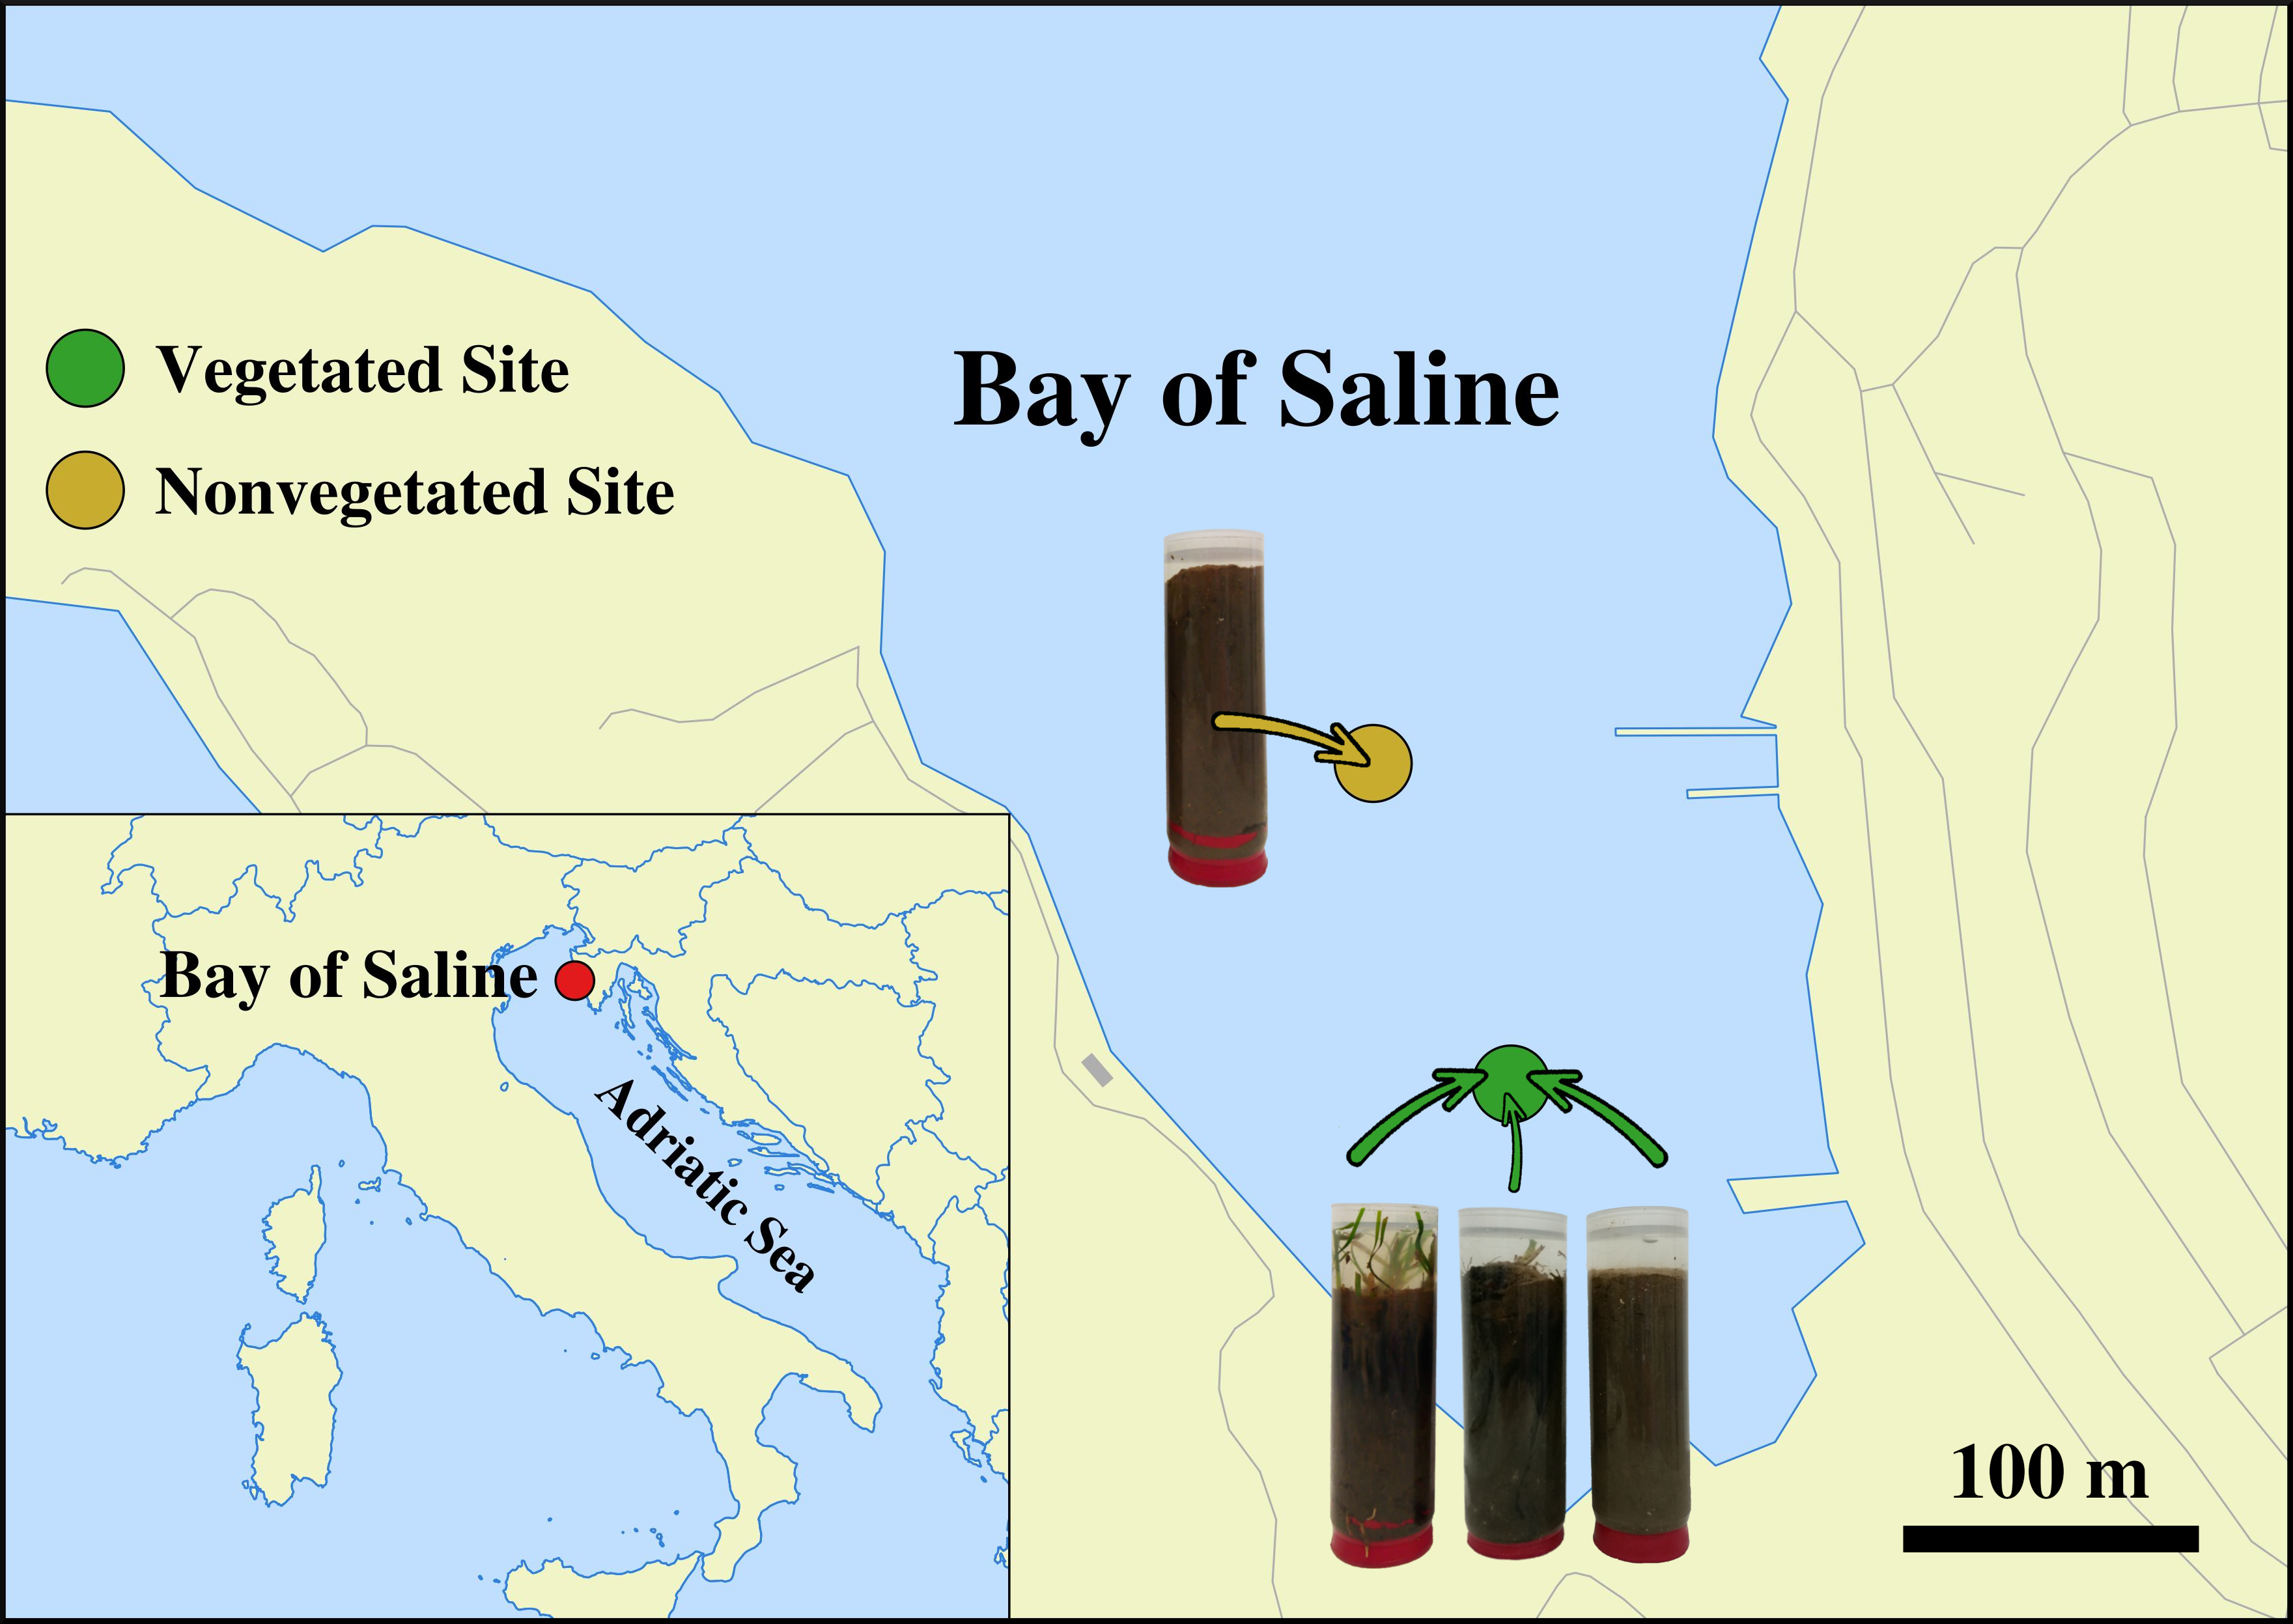
\includegraphics[width=1\linewidth]{../results/figures/map} 

}

\caption{Location of the vegetated (declining \textit{Cymodocea nodosa} meadow) and nonvegetated site in the Bay of Saline, northern Adriatic Sea (© OpenStreetMap contributors, www.openstreetmap.org/copyright).\label{map}}\label{fig:unnamed-chunk-1}
\end{figure}

\begin{figure}[H]

{\centering 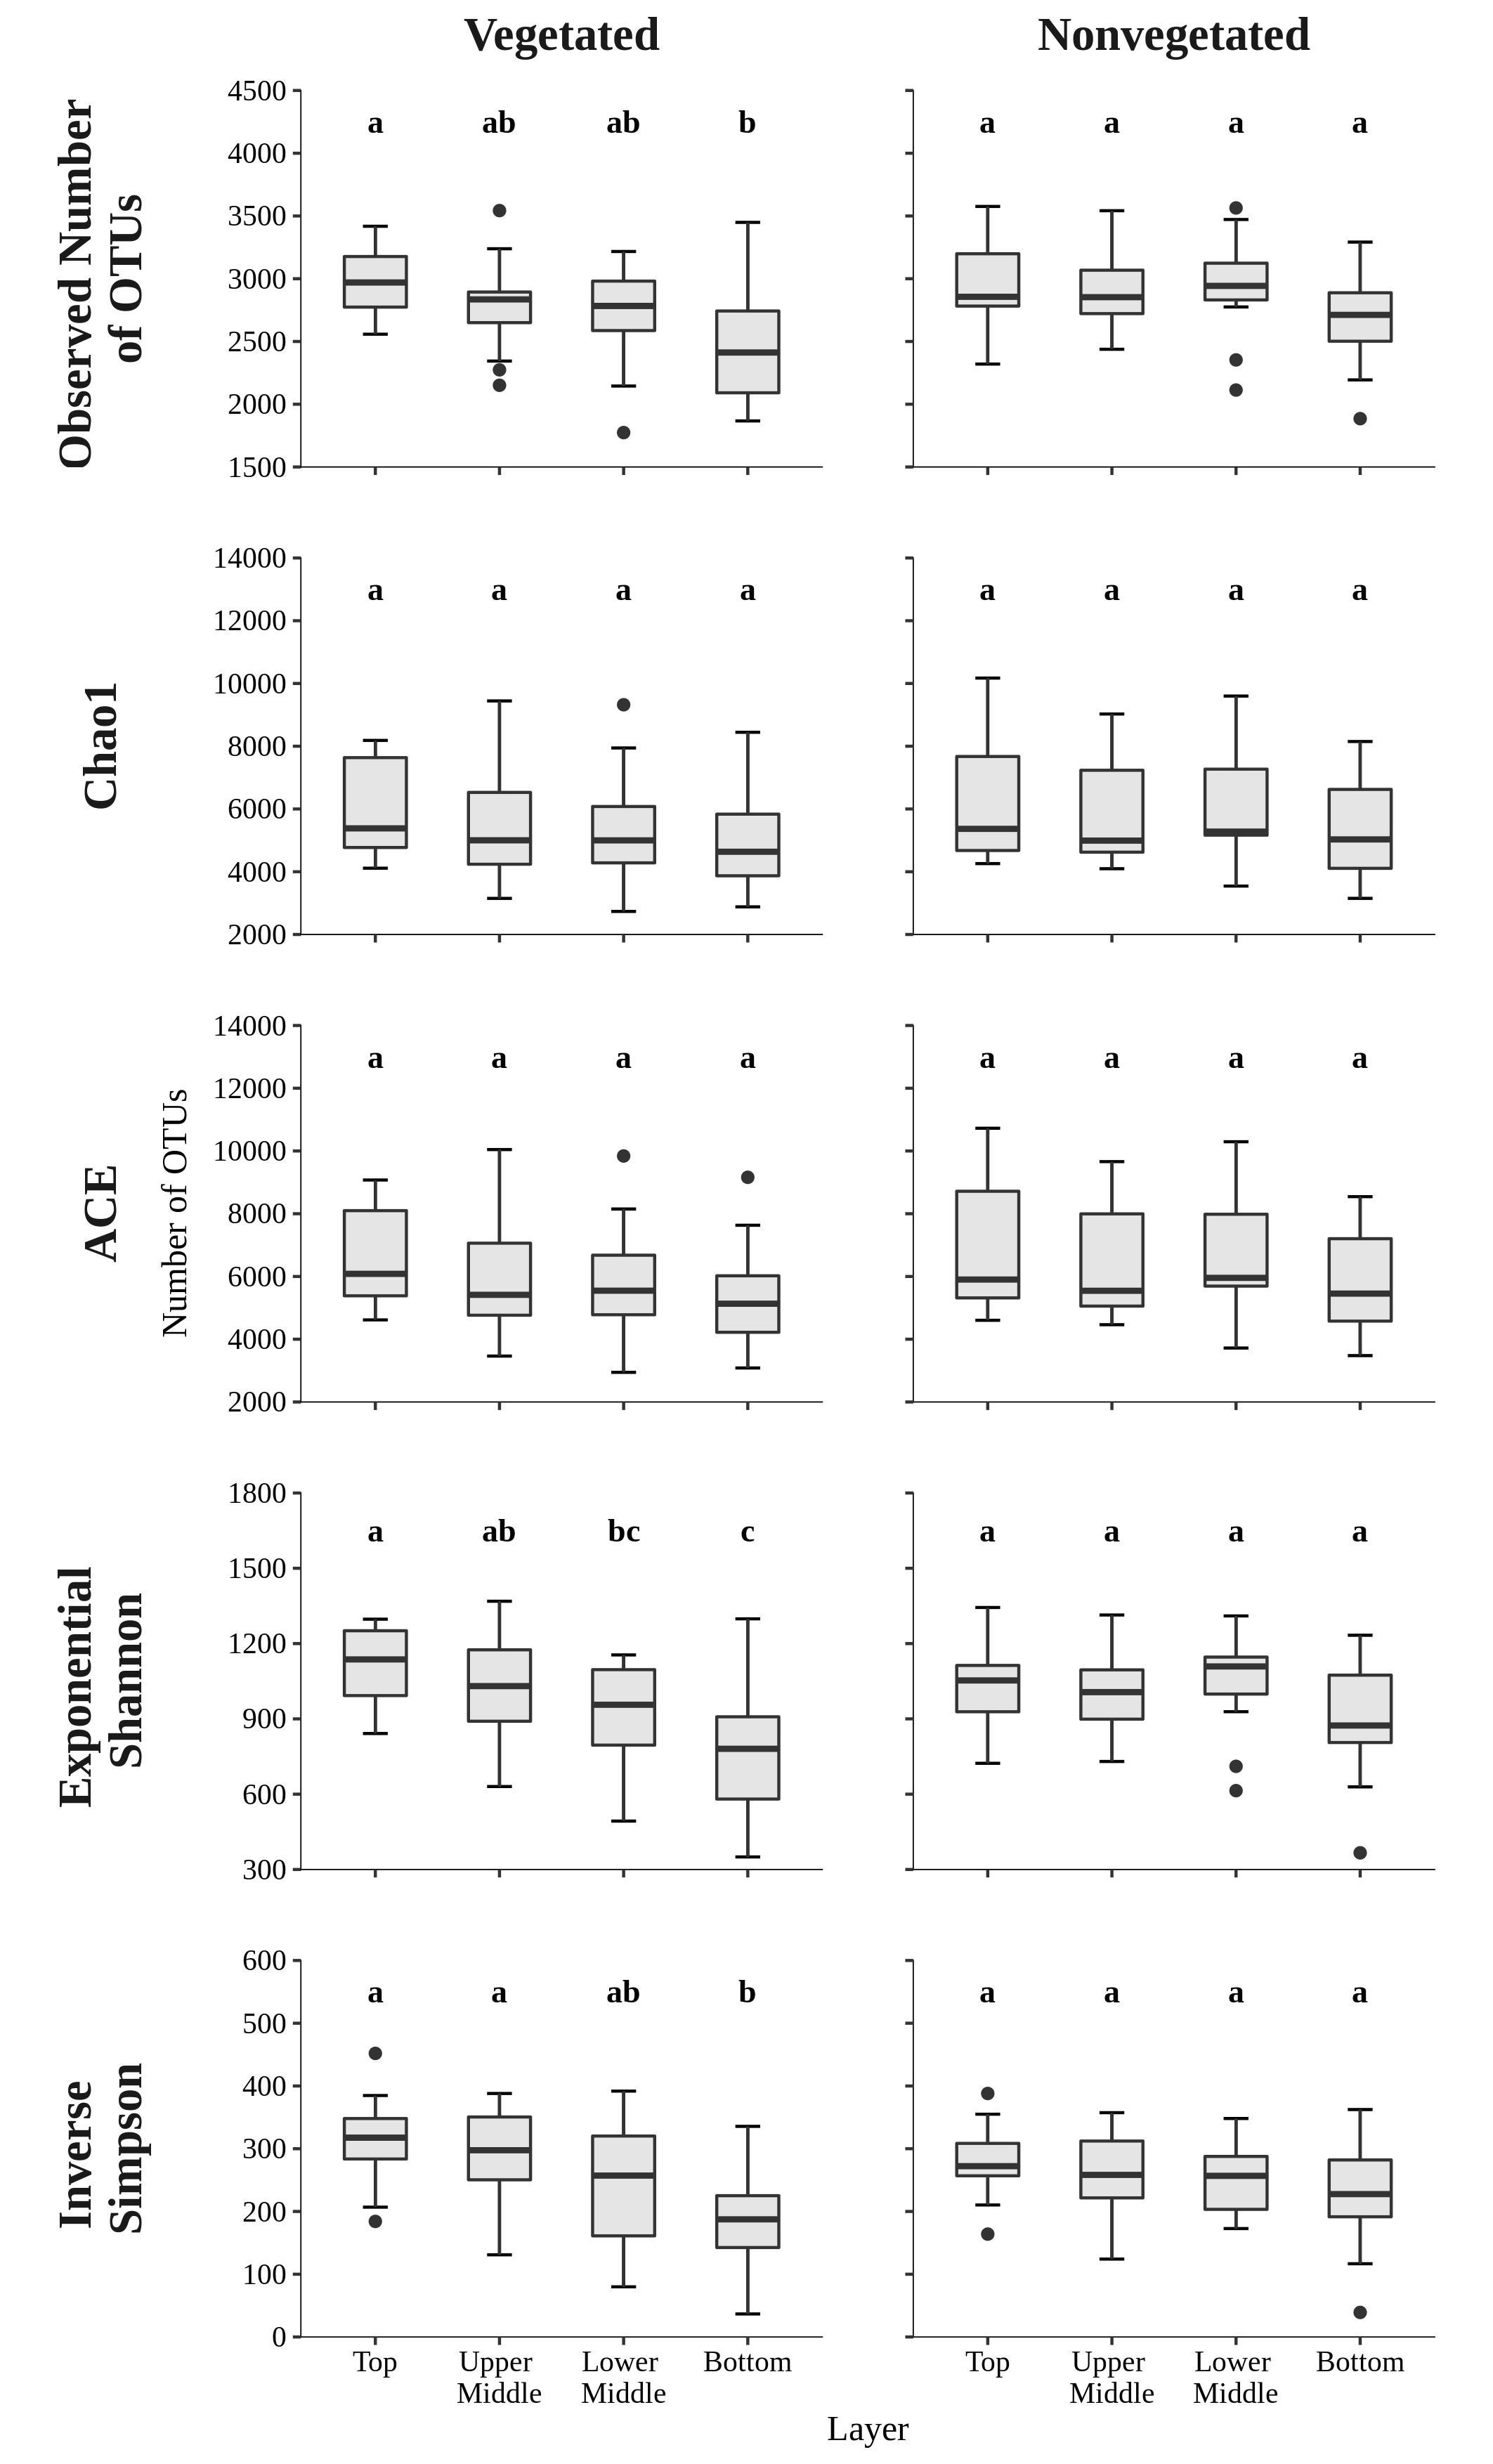
\includegraphics[width=0.7\linewidth]{../results/figures/calculators} 

}

\caption{The observed number of OTUs, Chao1, ACE, exponential of the Shannon diversity index, and Inverse Simpson diversity index of sediment microbial communities sampled in different sediment layers of the vegetated and nonvegetated site in the Bay of Saline.\label{calculators}}\label{fig:unnamed-chunk-2}
\end{figure}

\begin{figure}[H]

{\centering 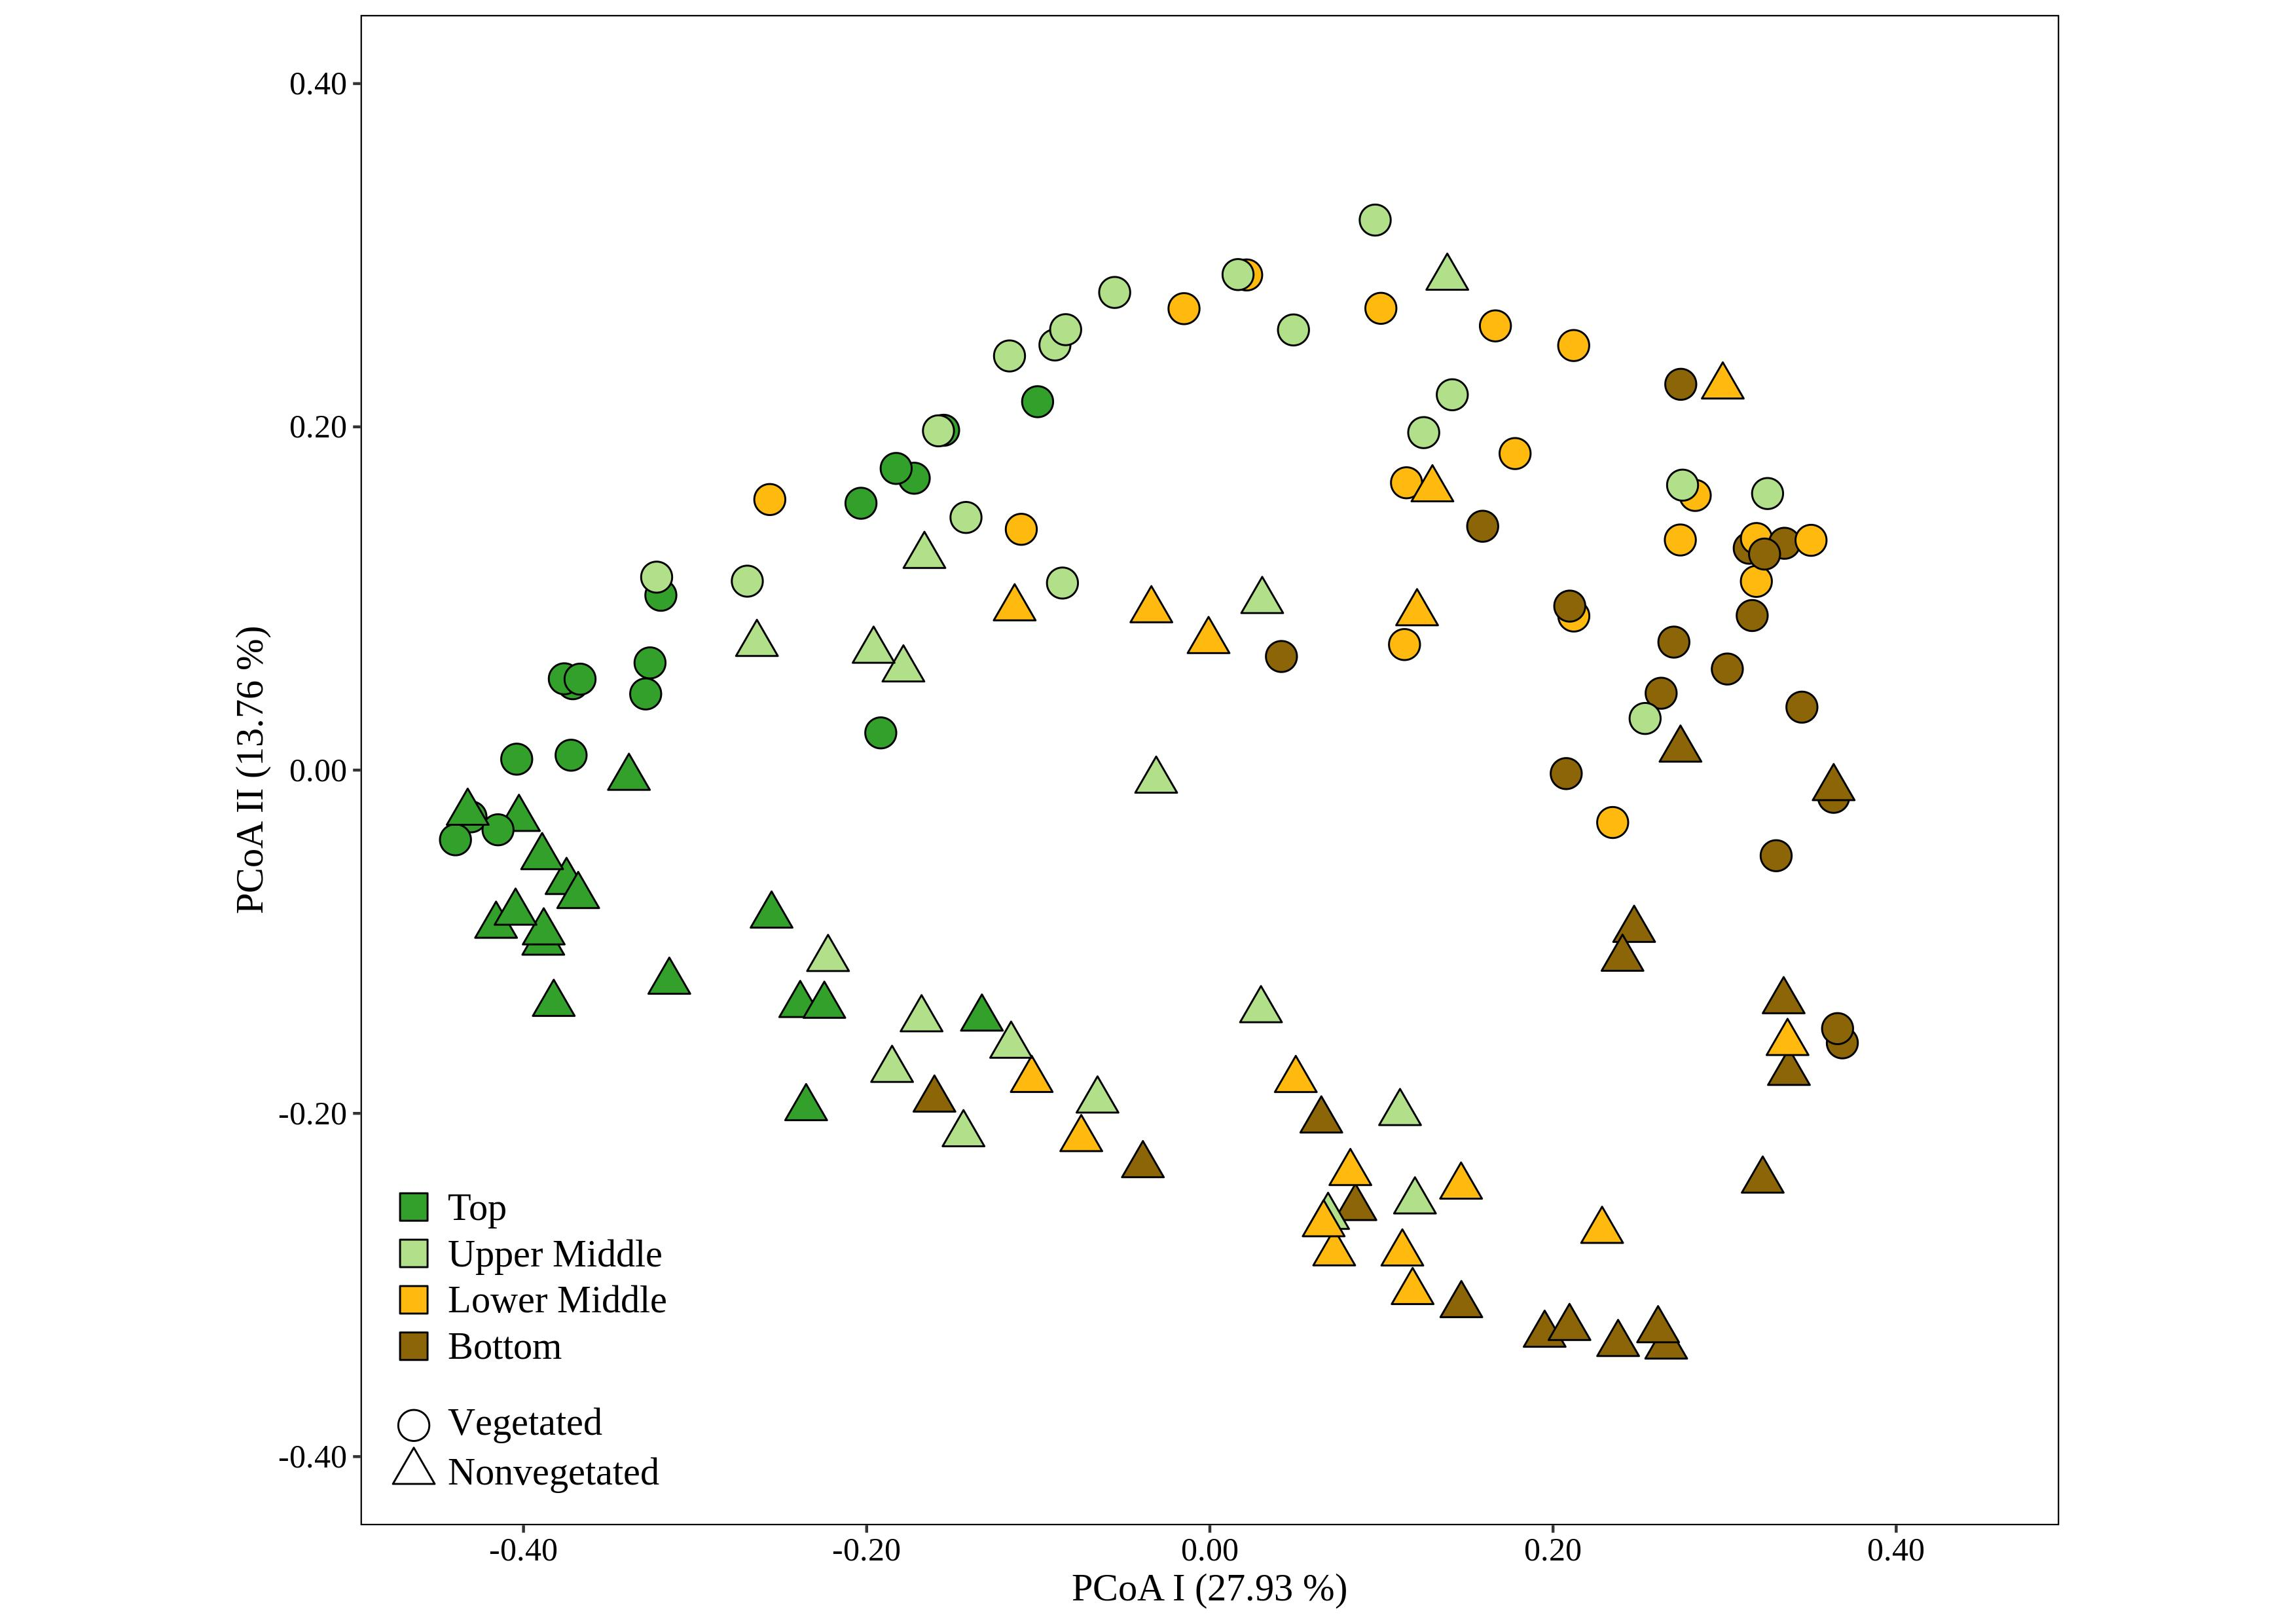
\includegraphics[width=0.9\linewidth]{../results/figures/pcoa_figure} 

}

\caption{Principal Coordinates Analysis (PCoA) of Bray-Curtis dissimilarities based on OTU abundances of sediment microbial communities sampled in the Bay of Saline. Samples from different sites are labelled with different symbols while samples from different sediment layers are indicated by colour. The proportion of explained variation by each axis is shown on the corresponding axis in parentheses.\label{pcoa_figure}}\label{fig:unnamed-chunk-3}
\end{figure}

\begin{figure}[H]

{\centering 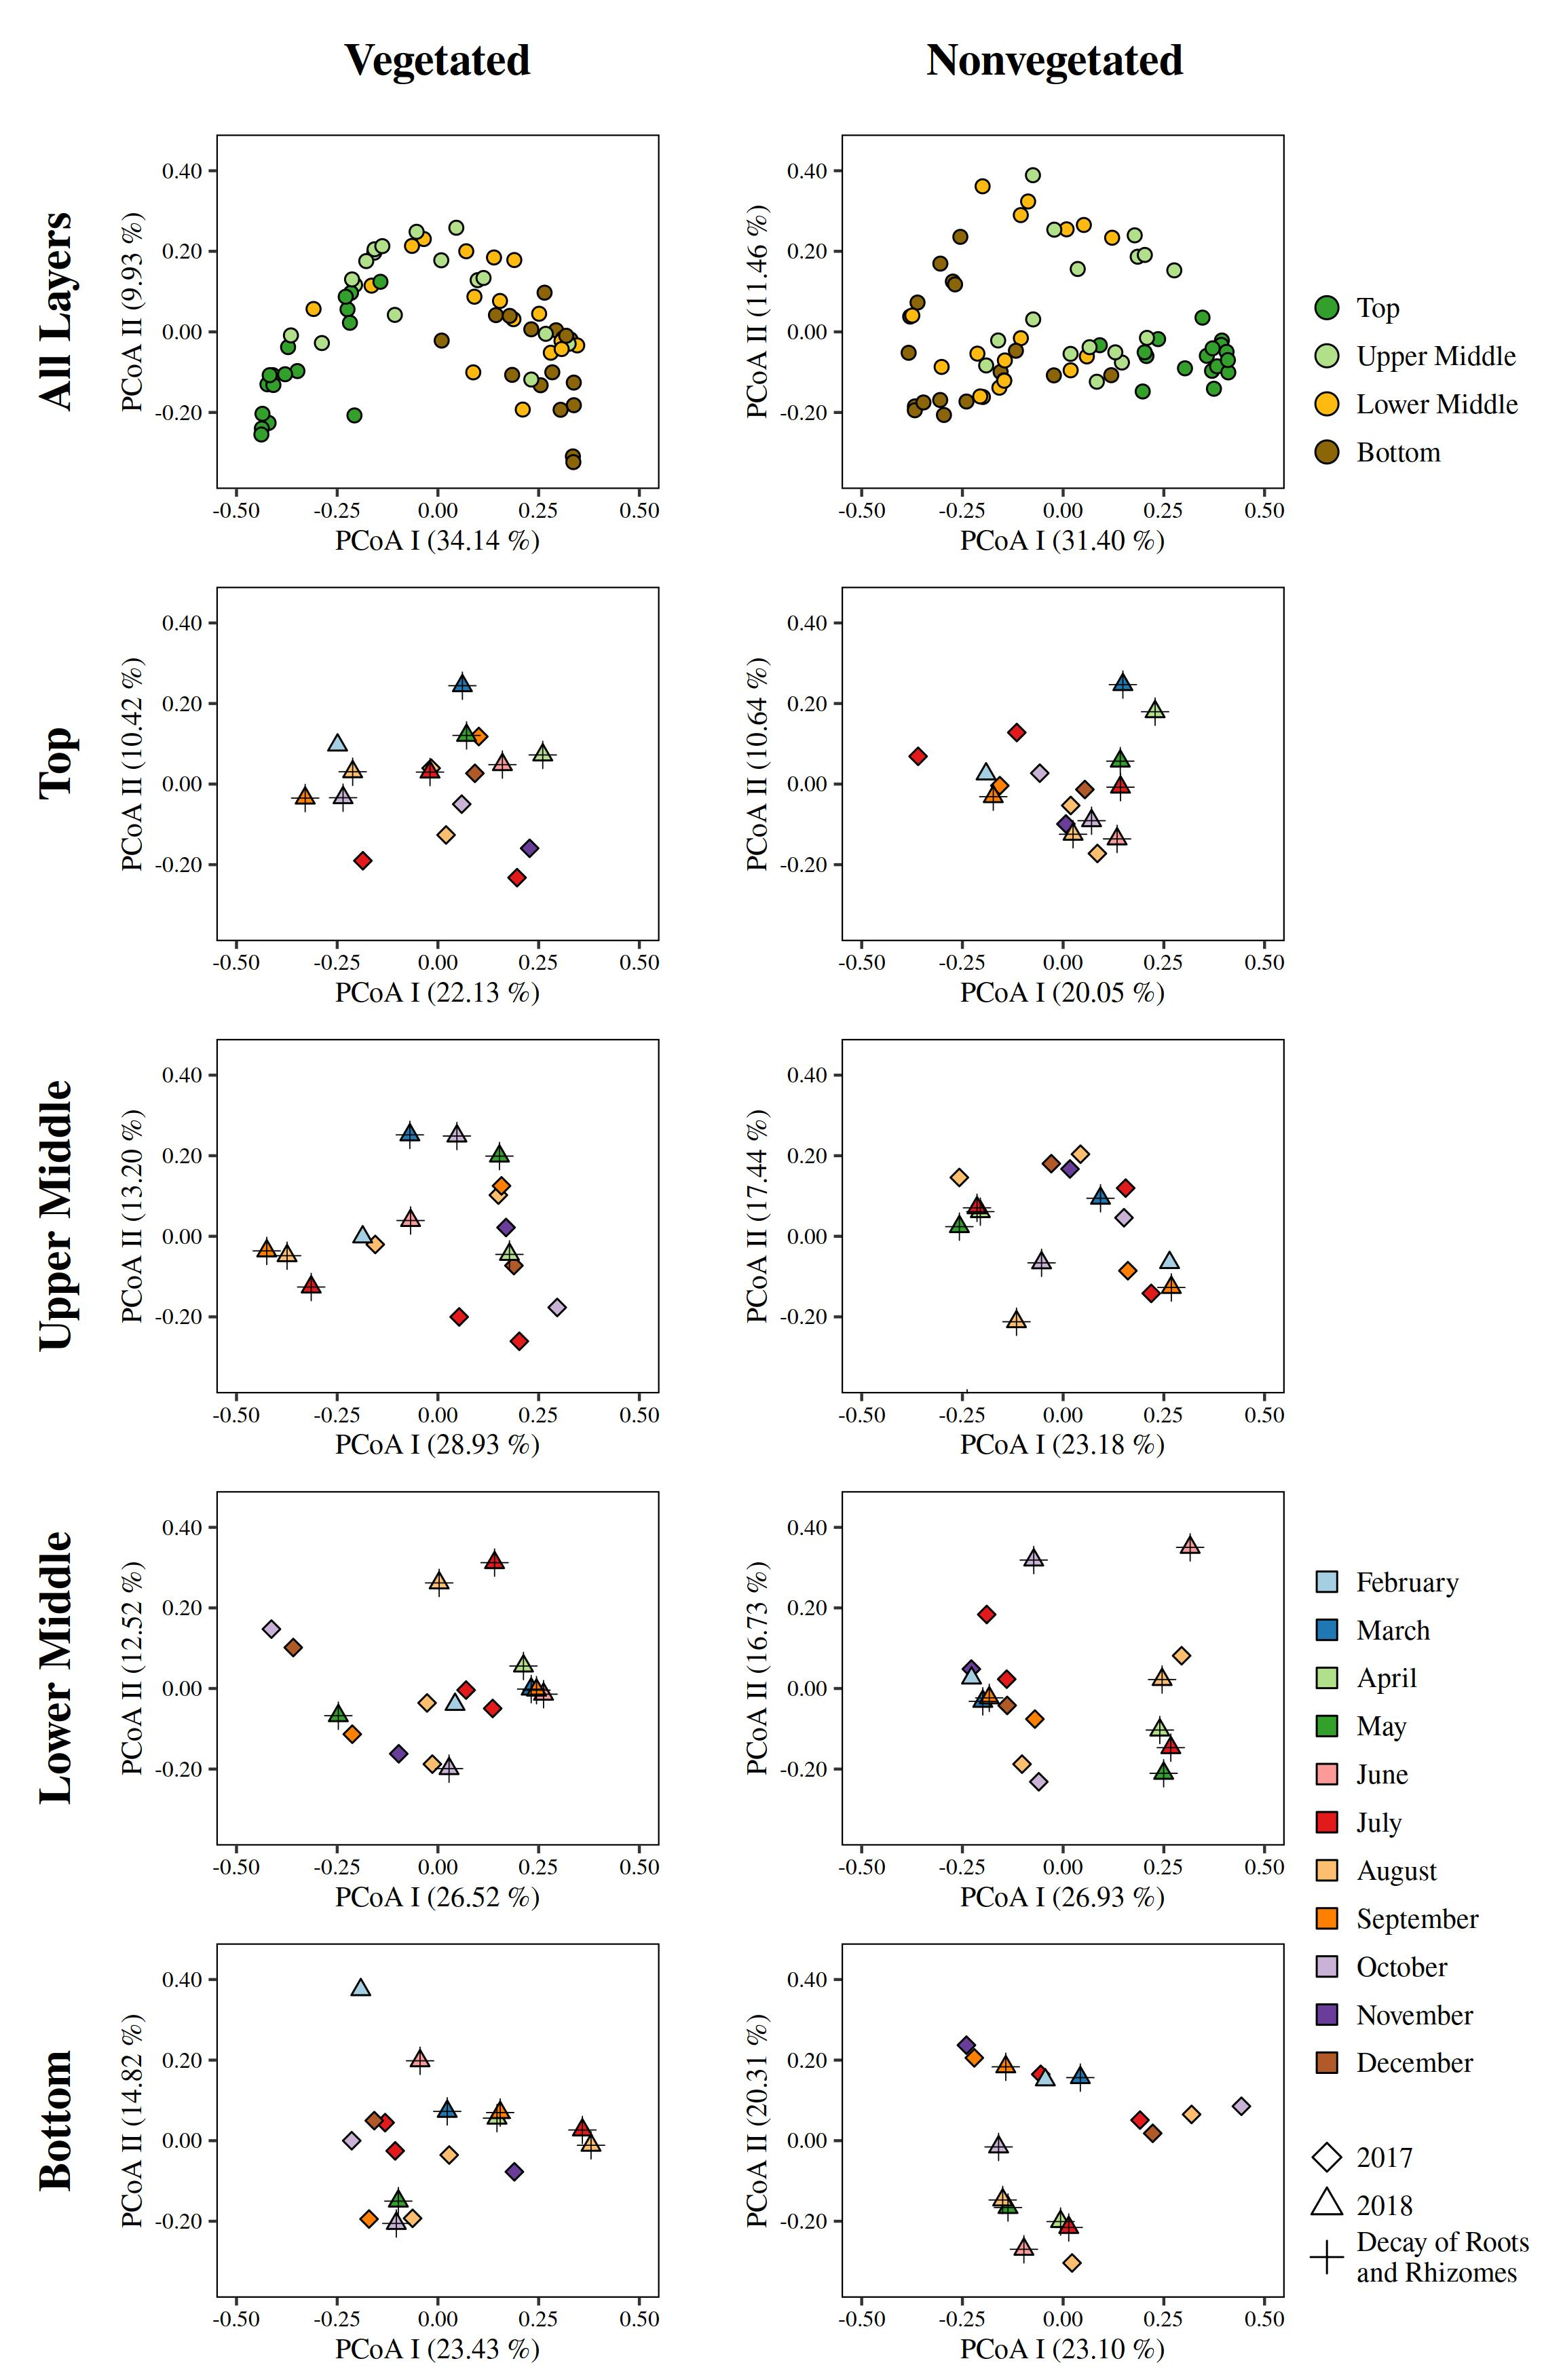
\includegraphics[width=0.8\linewidth]{../results/figures/pcoa_figure_areas_layers} 

}

\caption{Principal Coordinates Analyses (PCoA) of Bray-Curtis dissimilarities based on OTU abundances of sediment microbial communities, of all and individual sediment layers, sampled at the vegetated and nonvegetated site in the Bay of Saline. The proportion of explained variation by each axis is shown on the corresponding axis in parentheses.\label{pcoa_figure_areas_layers}}\label{fig:unnamed-chunk-4}
\end{figure}

\begin{figure}[H]

{\centering 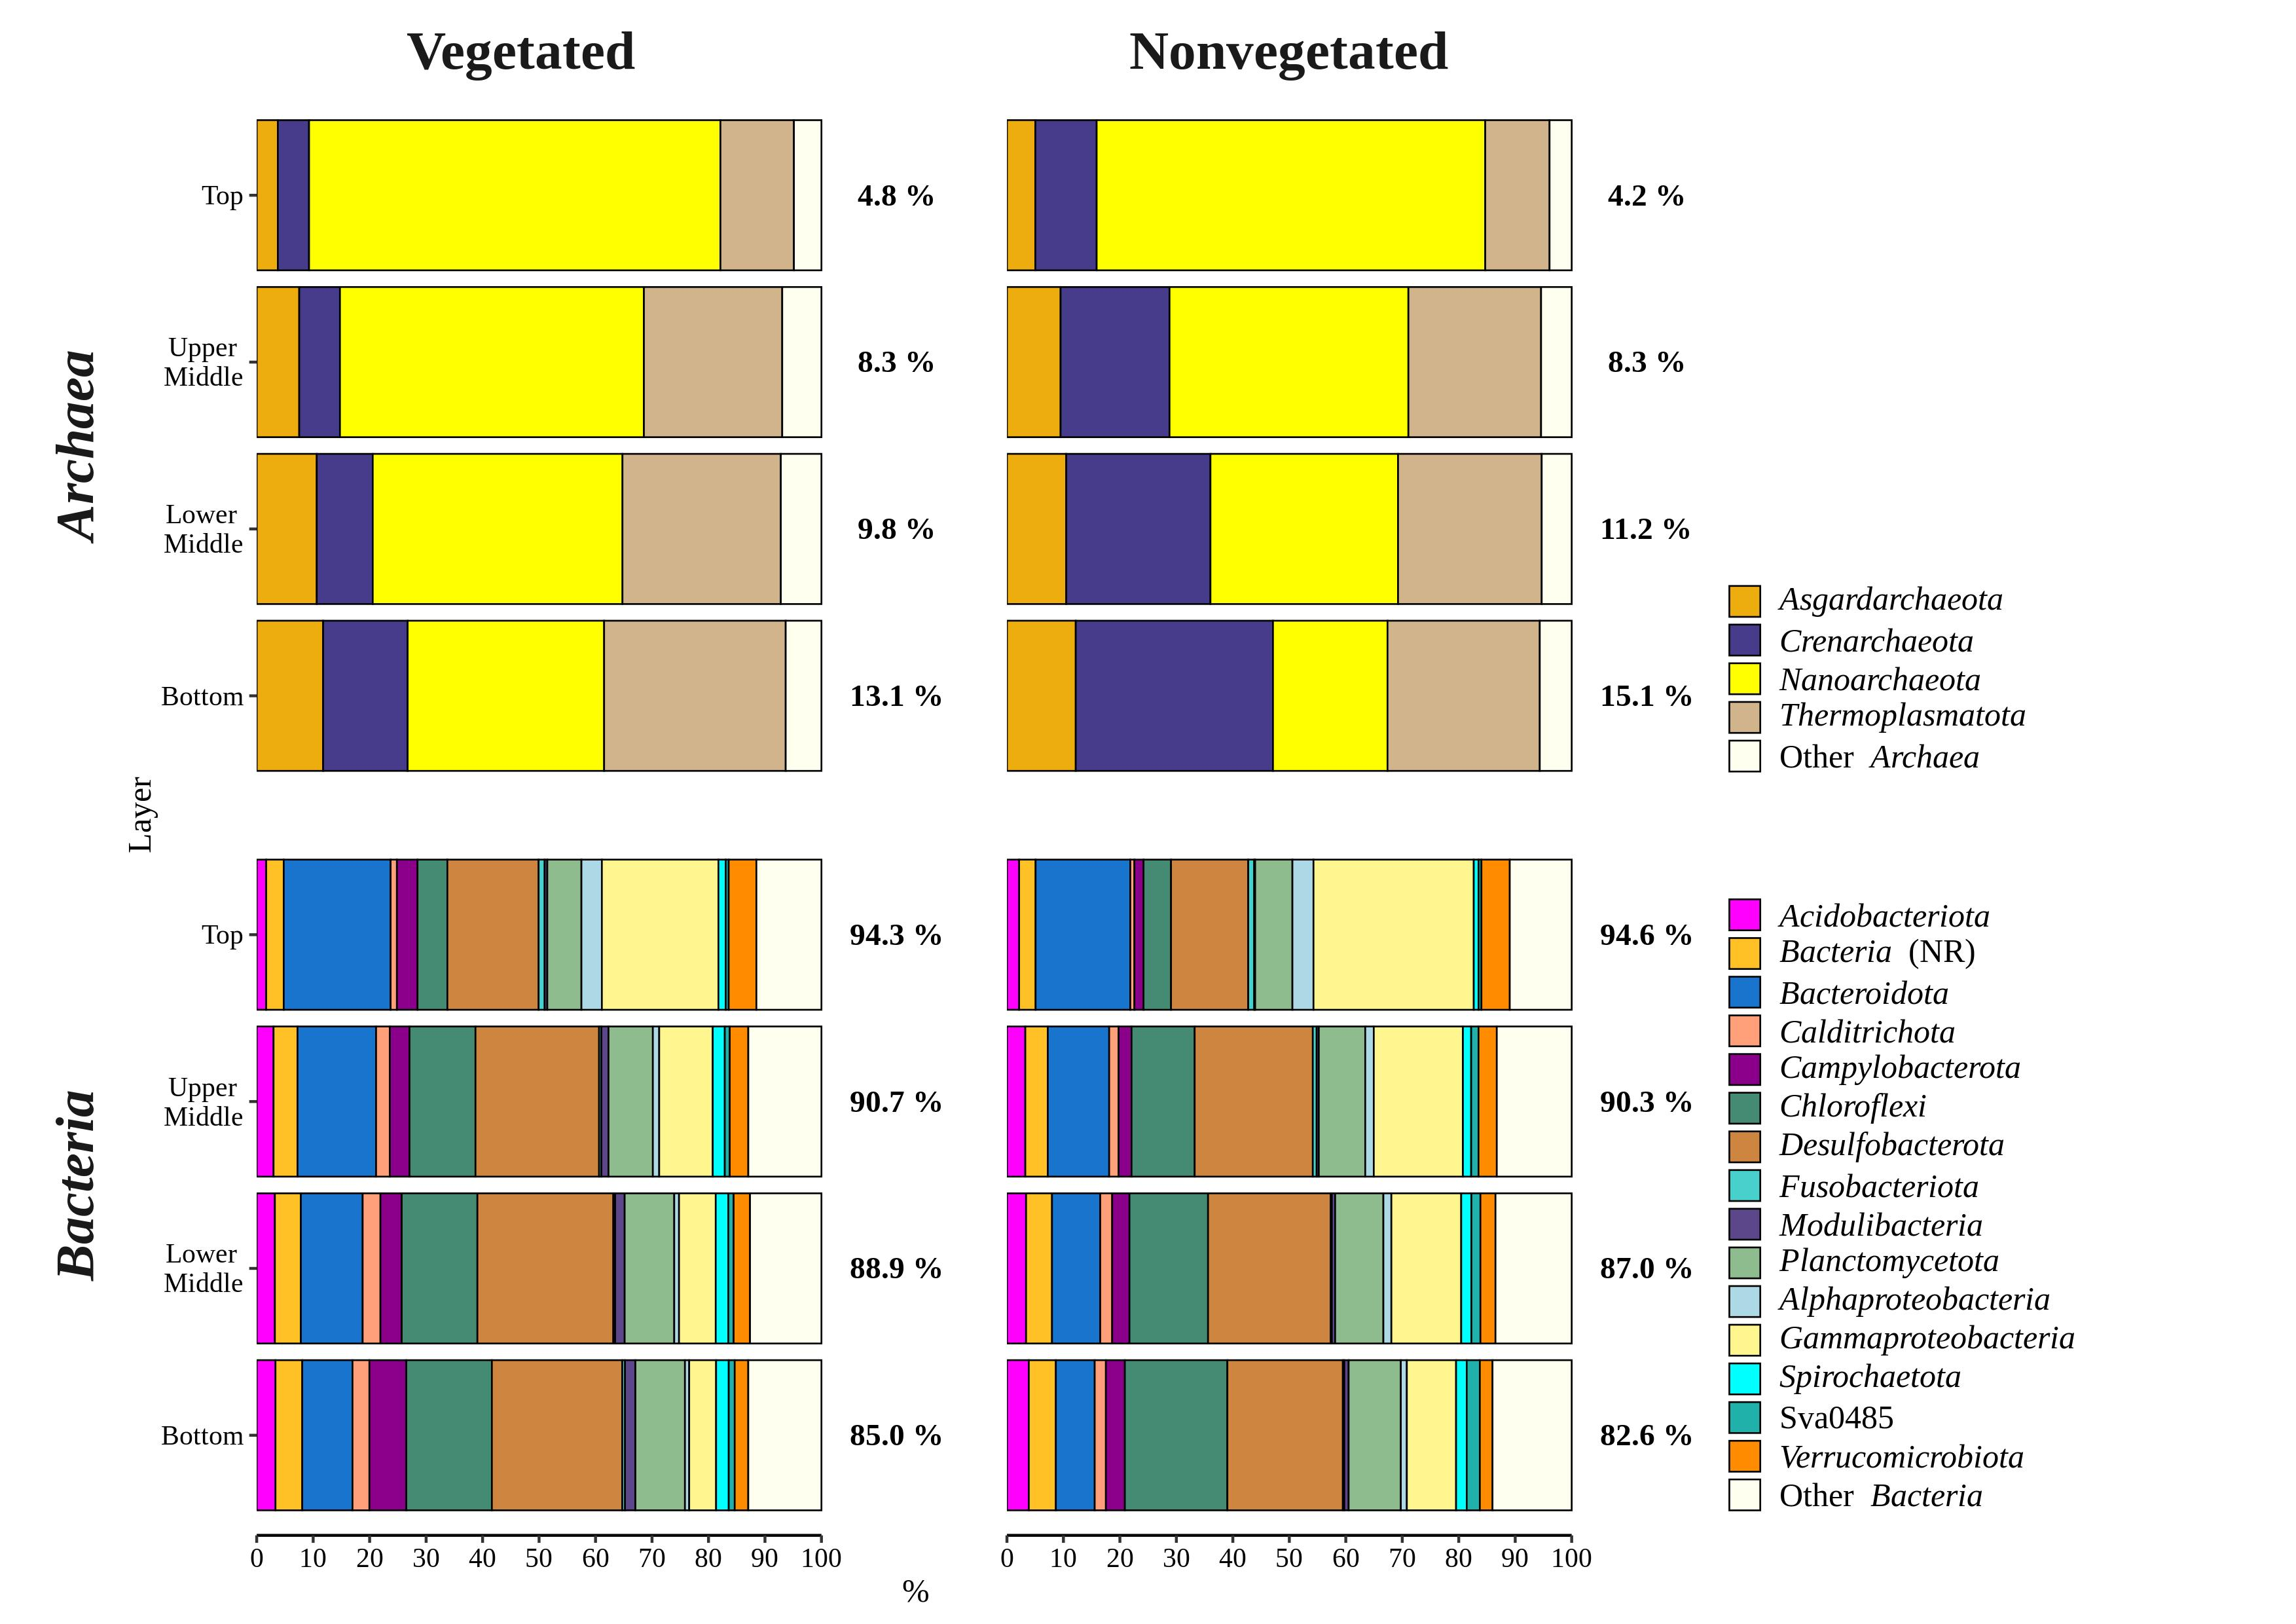
\includegraphics[width=1\linewidth]{../results/figures/community_barplot} 

}

\caption{Taxonomic classification and relative contribution of the most abundant  bacterial and archaeal ($\geq$ 3 \si{\percent}) sequences in sediment communities sampled at the vegetated and nonvegetated site in the Bay of Saline. NR -- sequences without known relatives\label{community_barplot}}\label{fig:unnamed-chunk-5}
\end{figure}

\begin{figure}[H]

{\centering 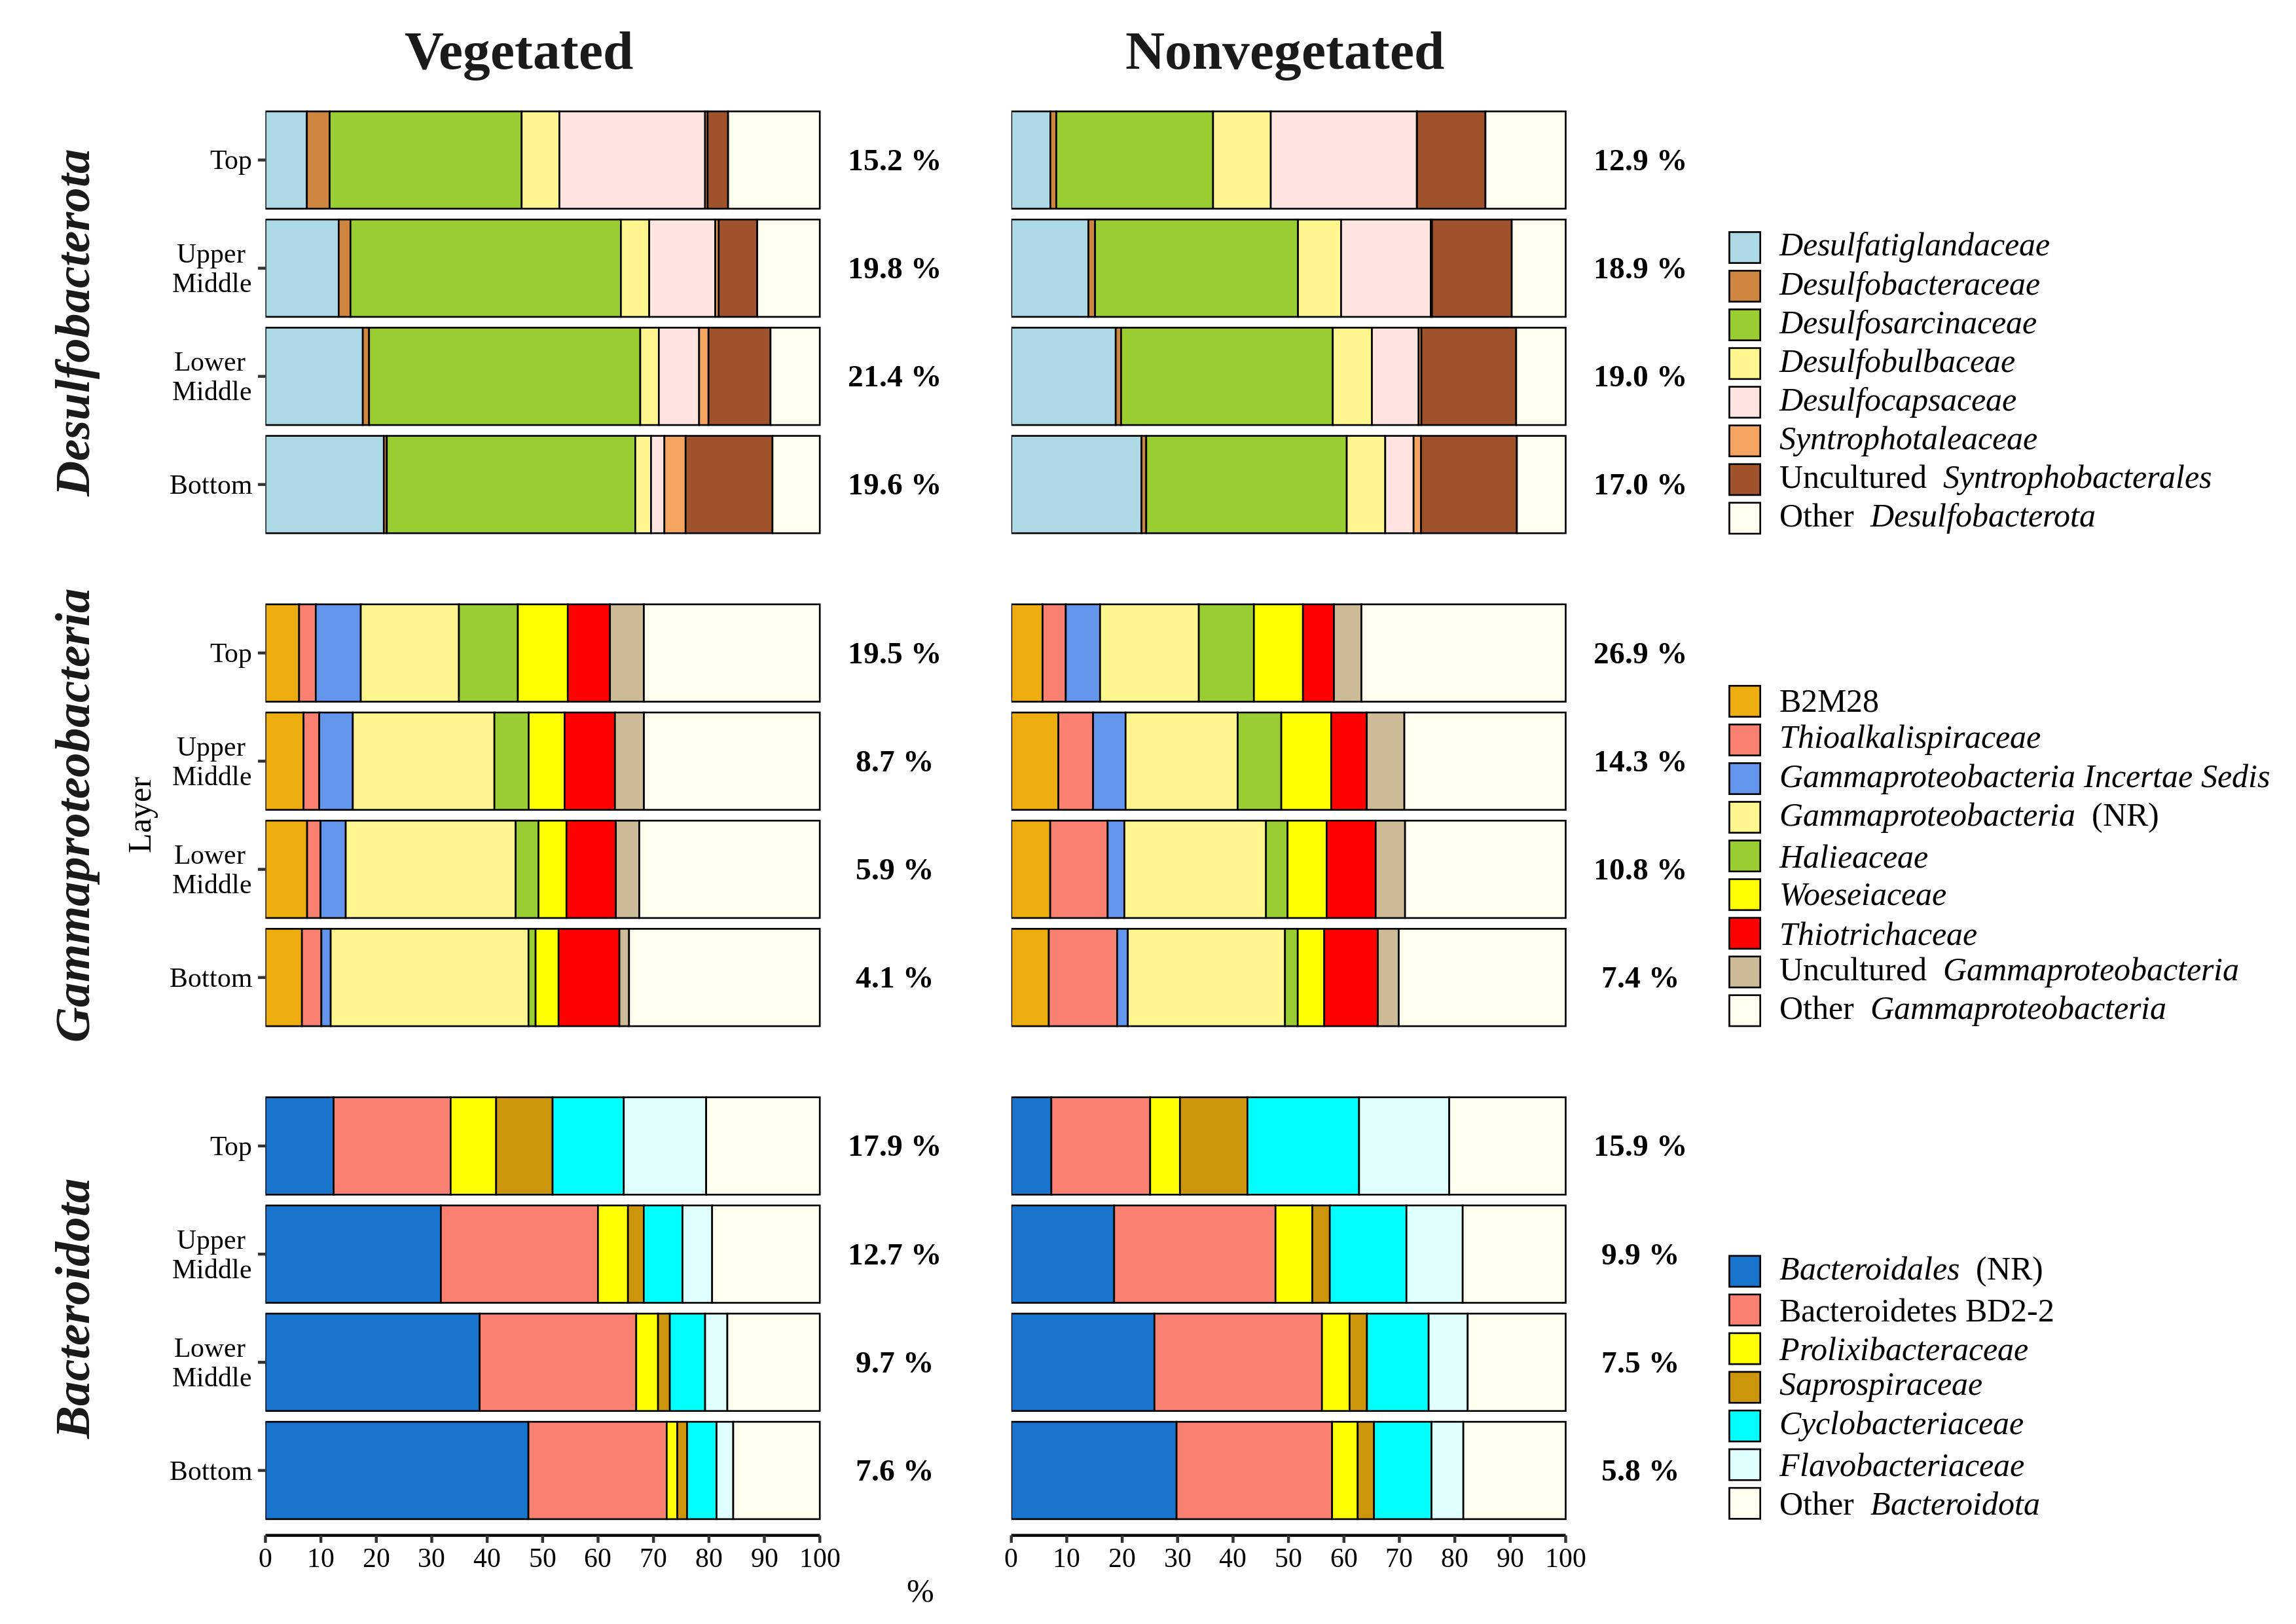
\includegraphics[width=1\linewidth]{../results/figures/community_barplot_major_1} 

}

\caption{Taxonomic classification and relative contribution of the most abundant ($\geq$ 2 \si{\percent}) taxonomic groups within \textit{Desulfobacterota}, \textit{Gammaproteobacteria}, and \textit{Bacteroidota} in sediment communities sampled at the vegetated and nonvegetated site in the Bay of Saline. NR -- sequences without known relatives\label{community_barplot_major1}}\label{fig:unnamed-chunk-6}
\end{figure}

\begin{figure}[H]

{\centering 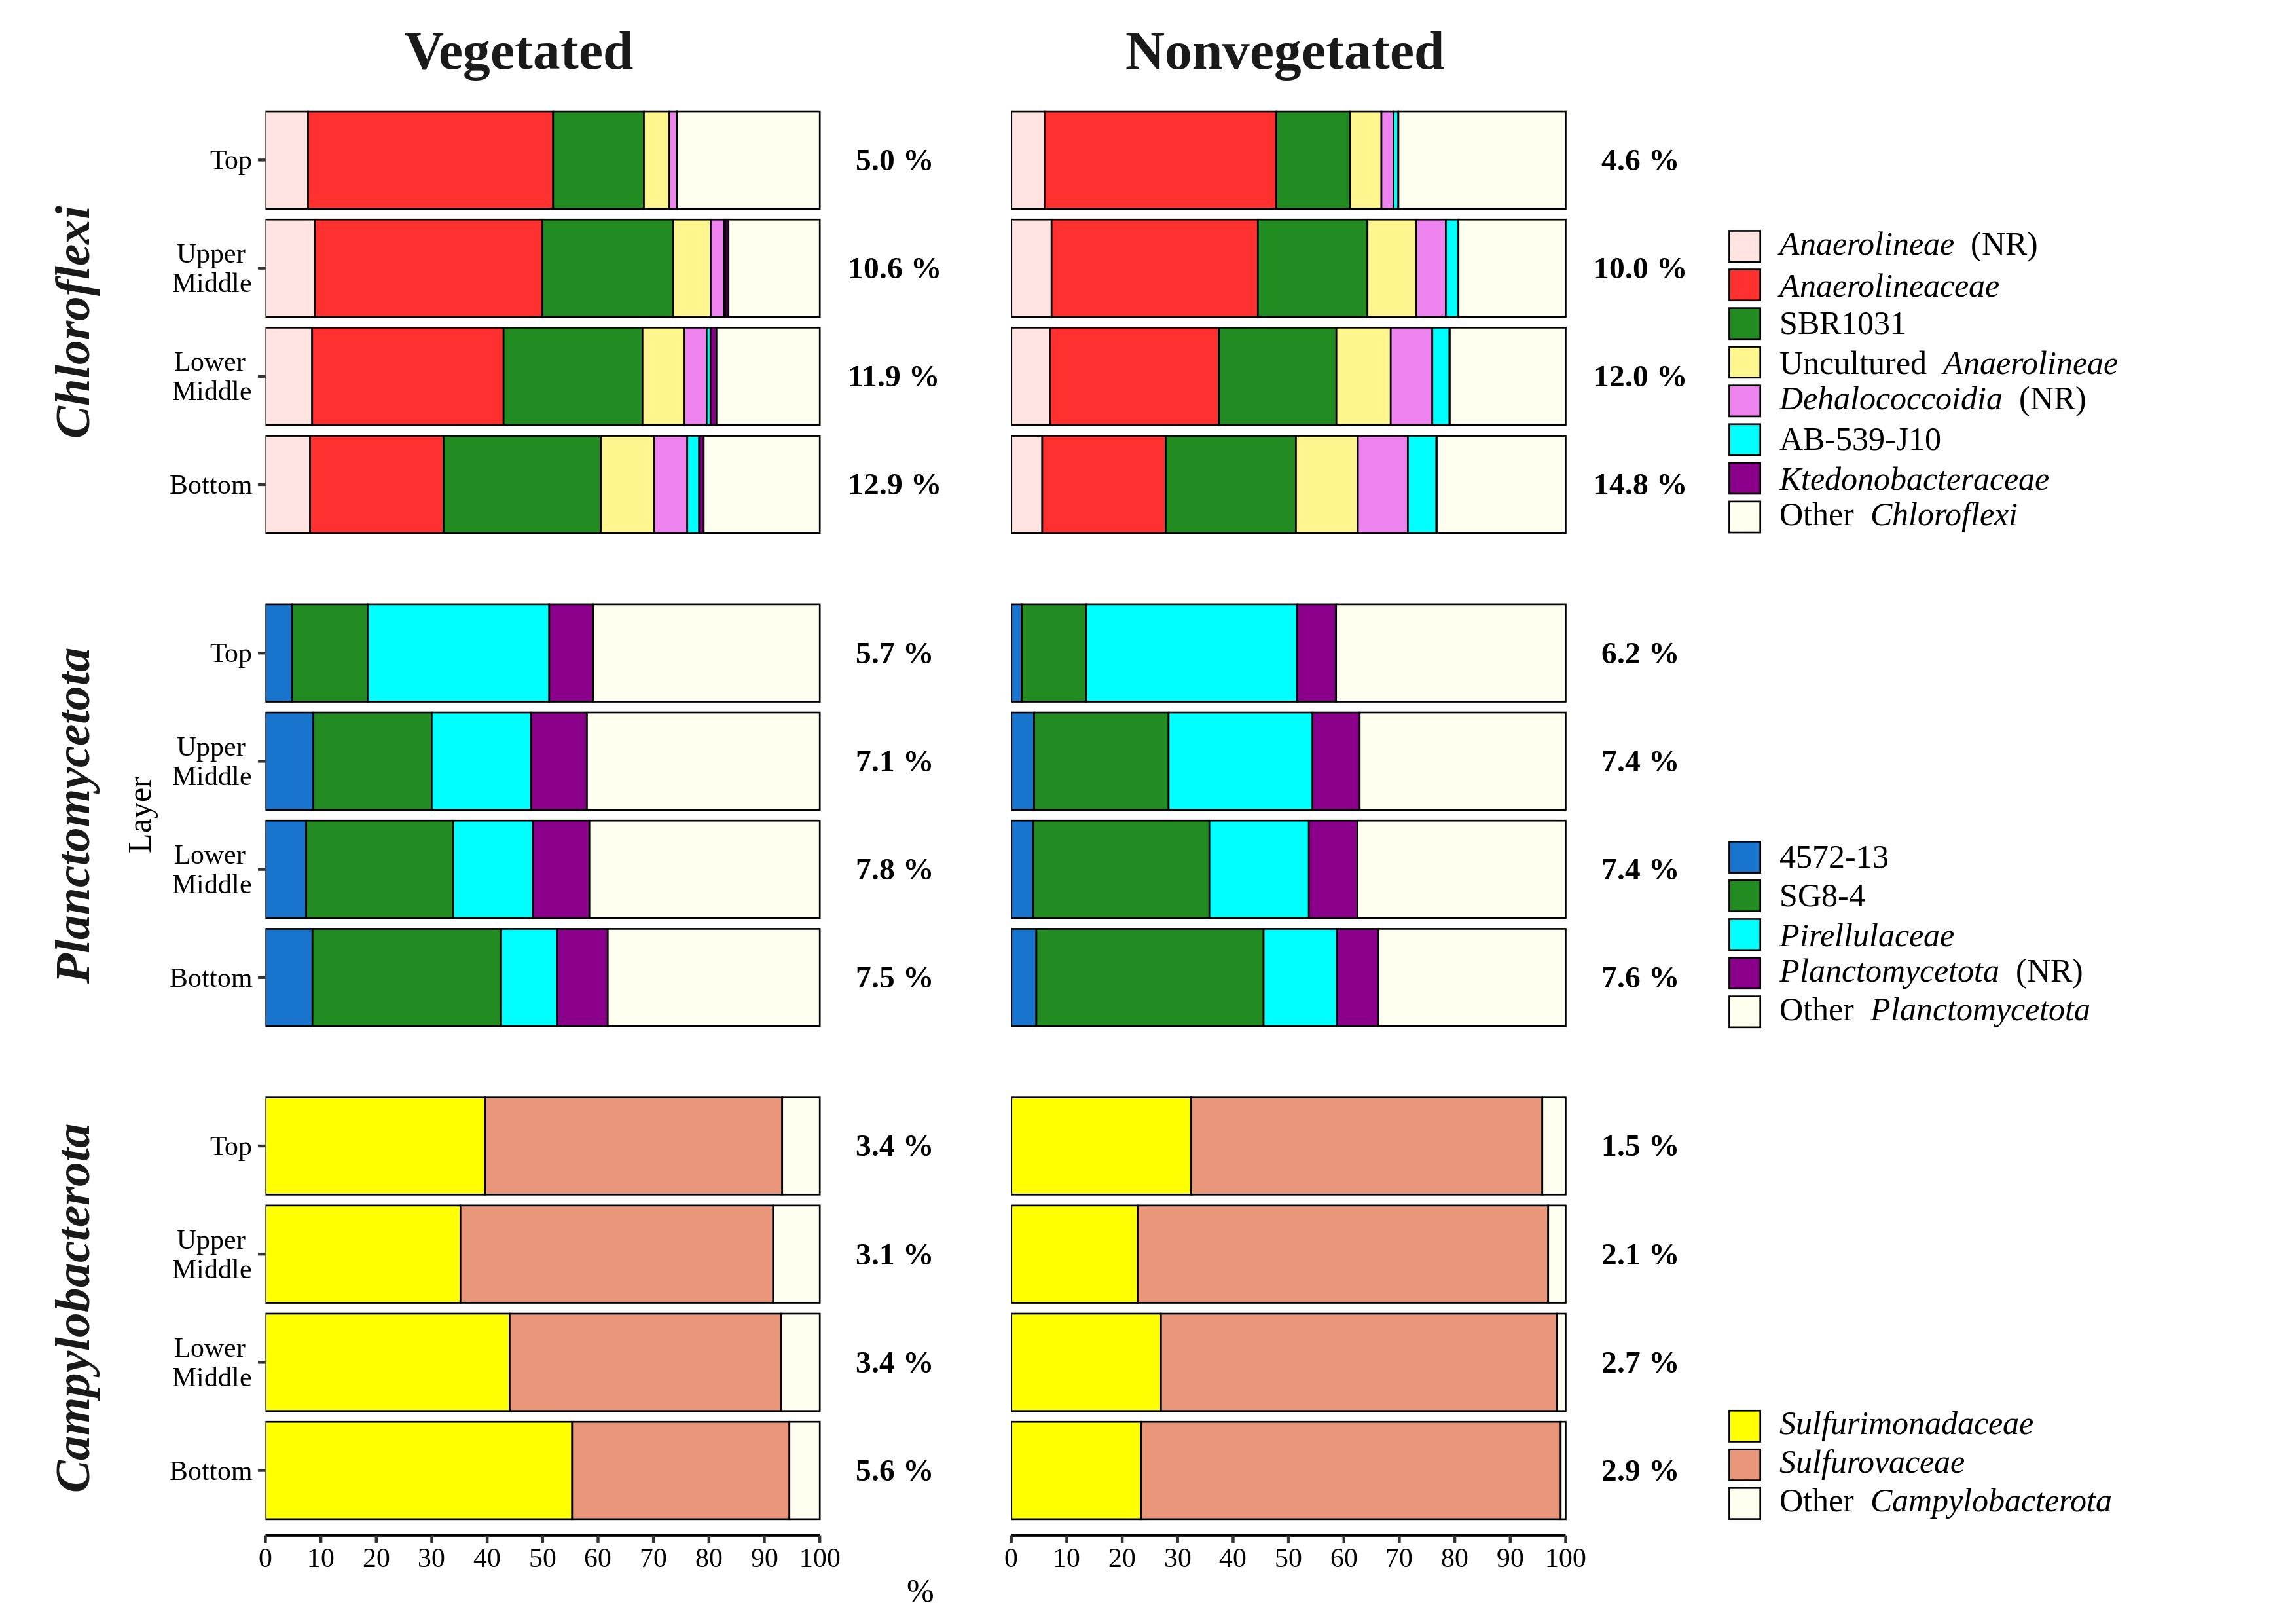
\includegraphics[width=1\linewidth]{../results/figures/community_barplot_major_2} 

}

\caption{Taxonomic classification and relative contribution of the most abundant ($\geq$ 1 \si{\percent}) taxonomic groups within \textit{Chloroflexi}, \textit{Planctomycetota}, and \textit{Campylobacterota} in sediment communities sampled at the vegetated and nonvegetated site in the Bay of Saline. NR -- sequences without known relatives\label{community_barplot_major2}}\label{fig:unnamed-chunk-7}
\end{figure}

\end{document}
